\documentclass[titlepage]{report}
\usepackage[ngerman]{babel}
\usepackage[backend=biber,style=numeric]{biblatex}
\addbibresource{literature.bib}
\usepackage{caption}
\usepackage{subcaption}
\usepackage{graphicx}
\usepackage[utf8]{inputenc}
\usepackage[T1]{fontenc}
\usepackage{url}
\usepackage{hyphenat}
\usepackage{glossaries}
\usepackage{array}
\usepackage{calc}
\usepackage{booktabs}
\usepackage{hyperref}
\usepackage{listings}
\usepackage{xcolor}
\usepackage{bytefield}
\usepackage{float}
\usepackage{eurosym}
\usepackage{tabu}
\usepackage{caption}
\lstset{%
    frame=tb,
    tabsize=4,
    numbers=left,
    breaklines=true,
}
\setcounter{biburllcpenalty}{9001}
\renewcommand{\lstlistingname}{Quelltext}
\renewcommand{\lstlistlistingname}{Quelltextverzeichnis}
\makeglossaries{}
\newglossaryentry{dns}
{%
    name={DNS},
    description={},
    first={Domain Name System (DNS)},
    long={Domain Name System}
}

\newglossaryentry{http}
{%
    name={HTTP},
    description={},
    first={Hypertext Transport Protocol (HTTP)},
    long={Hypertext Transport Protocol}

}
\newglossaryentry{https}
{%
    name={HTTPS},
    description={},
    first={Hypertext Transport Protocol Secure (HTTPS)},
    long={Hypertext Transport Protocol Secure}

}
\newglossaryentry{cifs}
{%
    name={CIFS},
    description={},
    first={Common Internet File System (CIFS)},
    long={Common Internet File System}

}
\newglossaryentry{voip}
{%
    name={VoIP},
    description={},
    first={Voice Over Internet Protocol (VoIP)},
    long={Voice Over Internet Protocol}

}
\newglossaryentry{tuc}
{%
    name={TU Clausthal},
    description={},
    first={Technische Universität Clausthal},
}
\newglossaryentry{efzn}
{%
    name={EFZN},
    description={},
    first={Energie-Forschungszentrum Niedersachsen (EFZN)},
    long={Energie-Forschungszentrum Niedersachsen}
}
\newglossaryentry{rfc}
{%
    name={RFC},
    description={},
    first={Request For Comments (RFC)},
    long={Request For Comments}
}

\title{Evaluierung eines Messpunkte-Clusters für Netzwerktests auf dem
Campus der TU Clausthal}
\author{Christian, Rebischke\\
\gls{tuc}\\
Rechenzentrum\\
Matrikelnummer: 432108 \\
Studiengang: Informatik (Bachelor) \\
Email: Christian.Rebischke@tu-clausthal.de}
\begin{document}
\maketitle
\chapter*{Danksagung}
Ich bedanke mich bei dem Rechenzentrum der \gls{tuc}, insbesondere bei
Dipl.\hyp{}Math. Christian Strauf. Das Thema dieser Bachelorarbeit
beruht auf seiner Idee und war mein Ansporn, mich mit diesem Thema näher
auseinanderzusetzen. Desweiteren danke ich Herrn Prof. Dr.\hyp{}Ing. Dr.
rer. nat. habil. Harald Richter für die Unterstützung aus akademischer
Seite. Besonderen Dank bekommt von mir auch die
Opensource\hyp{}Gemeinschaft.  Ohne die harte Arbeit der
Opensource\hyp{}Gemeinschaft würden die grundlegenden Werkzeuge, die
ich zur Vollendung dieser Bachelor-Arbeit benutzt habe, nicht
existieren. Besonders hilfreich waren das Softwarepaket \LaTeX{} und die
Zeichensoftware \emph{Draw IO} (\url{https://www.draw.io/}).
\chapter*{Eidesstattliche Erklärung}
Hiermit erkläre ich an Eides statt, dass ich die vorliegende Arbeit
selbstständig und nur unter Zuhilfenahme der ausgewiesenen Hilfsmittel
angefertig habe. Sämtliche Stellen der Arbeit, die im Wortlaut oder dem
Sinn nach anderen gedruckten oder im Internet verfügbaren Werken
entnommen sind, habe ich durch genaue Quellenangaben kenntlich gemacht.
Außerdem wurde diese Arbeit in gleicher oder ähnlicher Form noch keiner
anderen Prüfungsstelle im Sinne von \S 11 Absatz 5 lit. b) der
Allgemeinen Prüfungsordnung vorgelegt.
\\
\\
Clausthal-Zellerfeld, der \today
\\
\\
Christian Rebischke
\chapter*{Sperrvermerk}
Foobar Foobar Foobar
\\
\\
Clausthal-Zellerfeld, der \today
\\
\\
Christian Rebischke
\tableofcontents
\chapter*{Vorwort}
\addcontentsline{toc}{chapter}{Vorwort}
Es gibt nun mehr als 20 Jahren das Internet und keine Technologie
ist über so kurze Zeit so alltäglich geworden. Das Internet hat es
geschafft, Einzug zu erhalten in Arbeit, Privatleben und auch Forschung
und Lehre. Nahezu in allen wissenschaftlichen Diszplinen spielt das
Internet und die damit verknüpfte Informationstechnologie eine Rolle.
Sei es die Industrie 4.0 mit ihren cyber-physischen Systemen, dem
schnellen Abgleich von DNA-Informationen über das Netz in der
angewandten Biologie, dem Sammeln von Krankheitsdaten in der Medizin
oder das Verarbeiten von Datenmengen gigantischen Ausmaßes im
Finanzsektor. All diese Beispiele sind nur möglich durch immer größere
Technologiesprünge in der Informatik und dem immer größeren Ausbau des
Internets. Da ist es nicht verwunderlich, dass der UN-Menschenrechtsrat das
Internet zu einem Menschenrecht\cite{UNHRC} erklärt hat und umso weniger
verwunderlich ist es, dass die Vernetzung von Computersystemen auch auf
dem Campus der \gls{tuc} eine Rolle spielt,
nicht nur für Forschung und Lehre, sondern auch für den
täglichen Betrieb. Eine Schlüsselposition nimmt dabei das Rechenzentrum
der \gls{tuc} ein. Das Rechenzentrum bildet die
Basis für die Vernetzung der einzelnen Fakultäten untereinander, der
Vernetzung zwischen Fakultäten und Firmen aus der freien Wirtschaft,
sowie auch die Vernetzung zwischen der \gls{tuc}
und anderen Universitäten weltweit. Dementsprechend wichtig ist ein
stabiles Netz für den täglichen Betrieb. In dieser Bachelorarbeit widme
ich mich deshalb der technischen Umsetzung eines verteilten
Monitoring-Systems zur Überwachung der Netzwerkqualität zwischen
einzelnen Endpunkten und Kernsystemen, die für einen problemlosen
Netzbetrieb nötig sind. Das Rechenzentrum der \gls{tuc} dient bei dieser
Bachelorarbeit als Auftraggeber.
\chapter*{Problemstellung}
\addcontentsline{toc}{chapter}{Problemstellung}
Das Netz der \gls{tuc} erstreckt sich über mehrere
Standorte. Teilweise liegen diese Standorte nicht in Clausthal
selbst, wie beispielsweise das \gls{efzn} in Goslar. Dementsprechend
schwierig gestaltet sich die Wartung und der Betrieb
des Netzes. So kann auf Netzeinbrüche etwa nur reaktiv
nach Meldung des Problems reagiert werden. Es existiert
zwar ein Monitoring-System, welches die Verfügbarkeit von
einzelnen Diensten überprüft, jedoch erfolgt diese Messung
von einem Punkt aus und gibt binäre Statuswerte
zurück (Dienst läuft oder Dienst läuft nicht). Dementsprechend
fehlen Informationen um die Verfügbarkeit von Diensten und
deren vollständige Funktion von mehreren Messpunkten aus
zu garantieren. Beispielsweise ist es möglich, dass ein Dienst
zwar vom zentralen Monitoring-Server aus erreichbar ist, aber
aus einem einzelnen Institut der Zugriff auf den Dienst nur
eingeschränkt oder sogar gar nicht möglich ist. Das Rechenzentrum der
\gls{tuc} bietet mehrere Kerndienste an. Dazu
gehören:
\begin{itemize}
    \item \gls{dns}
    \item Diverse Webdienste basierend auf:
    \begin{itemize}
        \item \gls{http}
        \item \gls{https}
    \end{itemize}
    \item \gls{cifs}
    \item \gls{voip}
\end{itemize}

\autoref{fig:problemstellung} zeigt die aktuelle Netzstruktur der \gls{tuc}. Zu sehen
sind die drei \emph{Core\hyp{}Router}, welche auf die Gebiete
Rechenzentrum, Feldgraben und Tannenhöhe verteilt sind.
\emph{Core\hyp{}Router} stellen das Rückgrat, den Backbone, des Netzes
der \gls{tuc} dar und leiten den Datenverkehr zwischen den einzelnen am
Netz angeschlossenen Geräten. Sie trennen außerdem das Netz in logische
Abschnitte. Zu sehen ist ebenfalls das aktuell existierende
Monitoring-System, welches einzelne Kerndienste überwacht. Diese
Kerndienste und das aktuelle Monitoring-System sind im Rechenzentrum
beheimatet. Dadurch entsteht eine physikalische und auch logische Nähe
der Systeme. Durch diese Nähe verlässt der Datenverkehr, welcher die
Kerndienste überprüft, niemals das Rechenzentrum. Dies führt dazu, dass
einzelne Kerndienste zwar als in Betrieb und fehlerfrei angezeigt
werden, aber durchaus die Möglichkeit besteht, dass einzelne Dienste
nicht von jedem Rechner aus erreichbar sind. Da außerdem nur ein binärer
Zustand ermittelt wird, ist unklar, wie groß die Latenz zwischen den
Diensten und den jeweiligen Endkunden ist. Diese Latenz ist allerdings
entscheidend und hat Einfluss auf die Nutzererfahrung der Endkunden.
Besonders Dienste wie \gls{dns} sind auf schnelle Verbindungen
angewiesen. Eine zu hohe Latenz zwischen einem Client und dem Dienst
führt unweigerlich zu für den Nutzer spürbaren Konsequenzen (zum
Beispiel zu verzögerten Seitenaufrufe beim Web-Browsing). Noch mehr ins
Gewicht fallen Latenzen bei \gls{voip}, dort sind Latenzen oder ein
Jitter (die Varianz der Laufzeit der Datenpakete\cite{JITTERWIKI})
leicht auszumachen. Was fehlt, ist ein Netz aus verteilten Messpunkten,
das es ermöglicht, die Erreichbarkeit einzelner Dienste periodisch und
über einen längeren Zeitraum zu beobachten (siehe \autoref{fig:problemloesung}). Dies
hätte mehrere Vorteile: Zum einen ließe sich so der Zustand des
Campus-Netzwerks besser erfassen, da Tests nicht nur von einem zentralen
Monitoring-System aus gestartet werden. Zum anderen können die
gewonnenen Daten weiter verwertet, grafisch aufbereitet und zum Beispiel
für die Erstellung von Langzeitstatistiken über die Gesundheit des
Netzwerks genutzt werden.  Weiterhin könnten im Fall eines Ausfalls die
zuständigen Netzadministratoren benachrichtigt werden, im Idealfall
durch gewohnte Kommunikationswege wie Email. Außerdem wäre es durch
einen dezentralen Aufbau einfacher, das System beliebig zu skalieren
und auf Wachstum und Schrumpfen des Netzes zu reagieren. Mit dem Wandel
von einem zentralen zu einem dezentralen Monitoring-System entsteht
allerdings auch mehr Arbeitsaufwand, denn auch diese Systeme müssen
gewartet werden. Dies umfasst das Verwalten von Konfigurationsdateien,
das Aktualisieren und Installieren von Software und die Installation des
Grundsystems. Insgesamt lassen sich daraus folgende
Herausforderungen an diese Arbeit ableiten:

\begin{itemize}
    \item Es muss eine Hardware gefunden werden, welche sich
          als verteilter Messpunkt eignet.
    \item Es muss eine Monitoring\hyp{}Plattform gebaut oder eine
          vorhandene Monitoring\hyp{}Plattform erweitert werden, so dass
          sie den Anforderungen aus der
          Problemstellung gerecht wird.
    \item Es muss ein Modell für die gespeicherten Daten gefunden
          werden.
    \item Es muss ein Weg zur Datenvisualisierung gefunden werden.
    \item Das System muss horizontal skalierbar sein. Das heißt, es
          muss um Messpunkte erweiterbar sein.
    \item Das System muss bei wachsendem Komplexitätsgrad und Anzahl von
          Messpunkten steuerbar und kontrollierbar bleiben.
    \item Das System muss über Rechnernetze kommunizieren.
\end{itemize}

\begin{figure}[H]
    \centering
    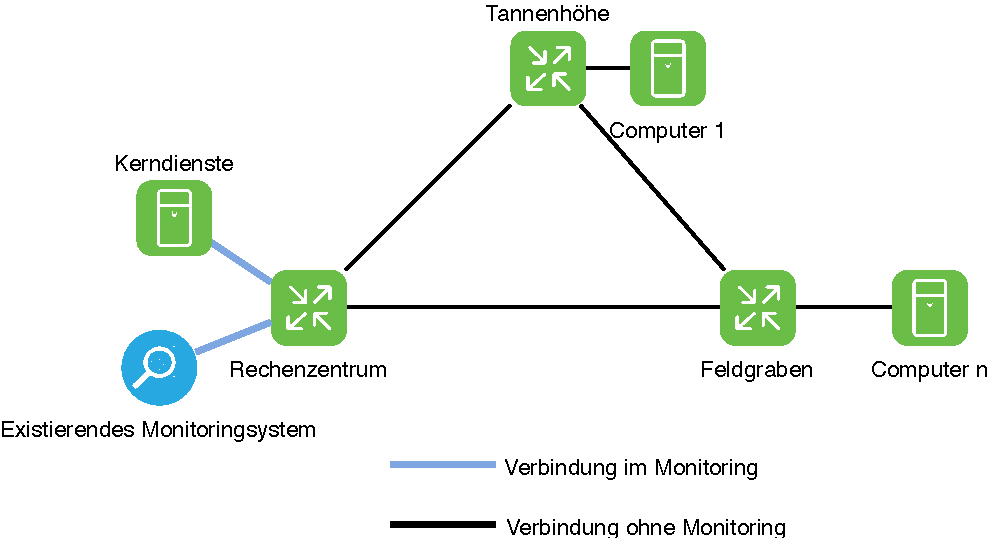
\includegraphics[width=1.0\textwidth]{figures/problemstellung.pdf}
    \caption{Veranschaulichung der Problemstellung}\label{fig:problemstellung}
\end{figure}
\begin{figure}[H]
    \centering
    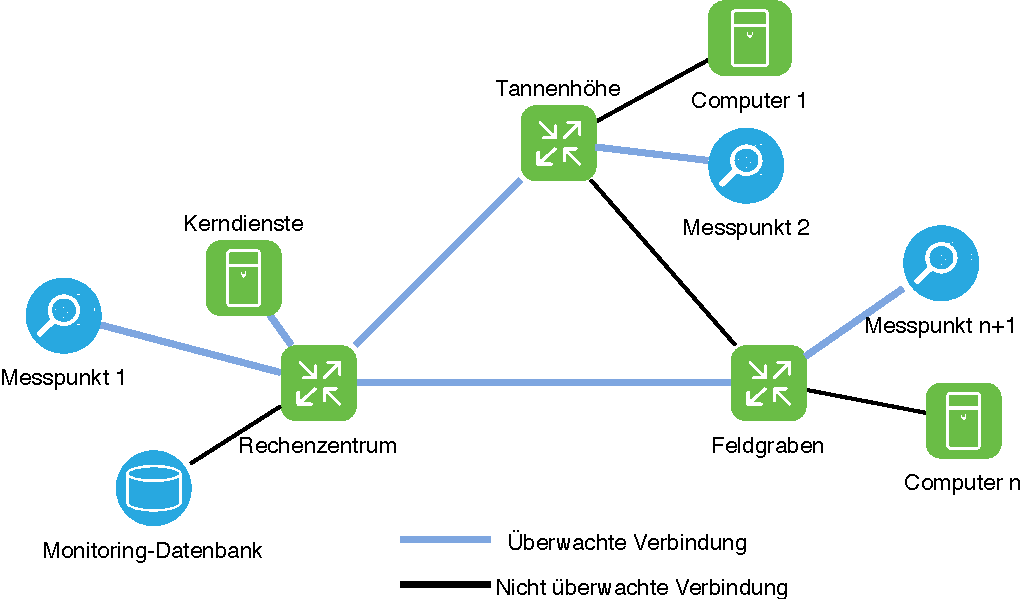
\includegraphics[width=1.0\textwidth]{figures/problemloesung.pdf}
    \caption{Veranschaulichung der Problemlösung}\label{fig:problemloesung}
\end{figure}
\chapter*{Technische Grundlagen}
\addcontentsline{toc}{chapter}{Technische Grundlagen}
In diesem Kapitel werden die für die Lösung des Problems nötigen
technischen Grundlagen erläutert. Außerdem werden die Fehlerfälle für
die einzelnen Protokolle definiert. Darunter fallen einige wichtige
Netzwerkprotokolle, sowie eine allgemeine Einführung in
Computernetzwerke.
\section*{Netzwerkgrundlagen}
\addcontentsline{toc}{section}{Netzwerkgrundlagen}
Um auf Basis der vorangegangenen Problemstellung eine Lösung zu
erarbeiten, ist es notwendig, einen groben Überblick über die Grundlagen
von Computernetzwerken zu bekommen. Als Basis dafür dient das \gls{osi}. Das
\gls{osi} ist de facto das bis heute gängige Referenzmodell, wenn es
darum geht, mehrere Systeme miteinander zu vernetzen. Ein solches System
wird \emph{offenes System} genannt, wenn es den im \gls{osi}
spezifizierten Standards entspricht\cite[Siehe Abschnitt
4.1.2]{ITUOSI}. Diese \emph{offenen Systemen} sind mit einem physischen
Medium verbunden und bilden so ein Computernetzwerk. \autoref{fig:opensystems}
zeigt eine solche Verbindung mehrerer \emph{offener Systeme}.
\begin{figure}[H]
    \centering
    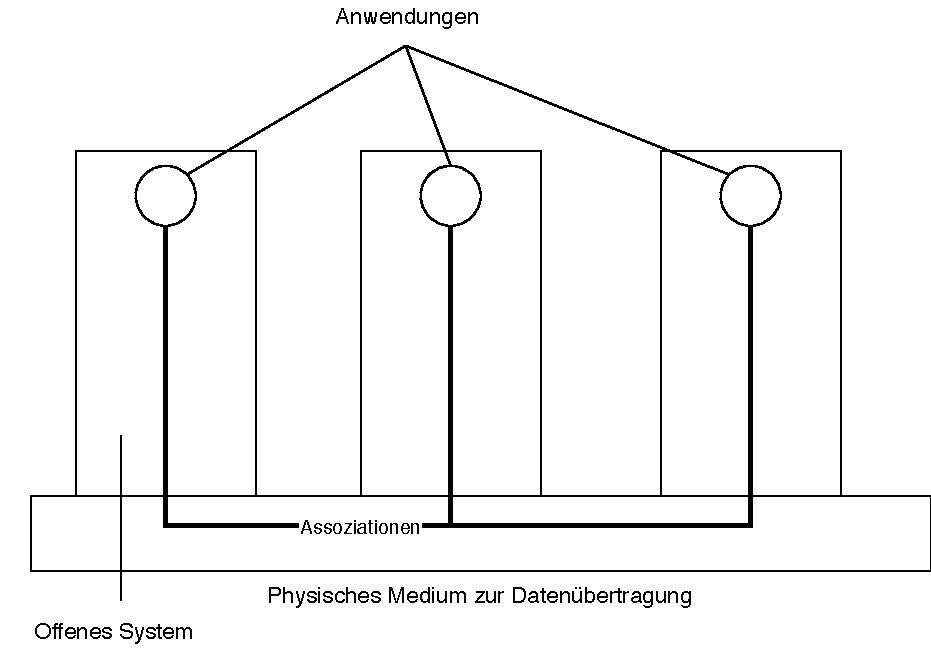
\includegraphics[width=0.8\textwidth]{figures/open_systems.pdf}
    \caption{Veranschaulichung der Assoziationen verschiedenener offener
    Systeme mit diversen Anwendungen über ein physisches Medium}\label{fig:opensystems}
\end{figure}
Innerhalb eines dieser \emph{offener Systeme} sind sieben
Netzwerkschichten oder auch \emph{OSI-Schichten} definiert\cite[Siehe
Abschnitt 6.1.2]{ITUOSI}. Zur
Kommunikation zwischen zwei \emph{offenen Systemen} wird mindestens eine
Schicht durchlaufen, in den meisten Fällen jedoch mehrere Schichten.
\autoref{fig:osi} listet alle sieben Schichten, deren Protokolle,
Einheiten und Einordnung auf. Die Funktionsweise des \gls{osi} lässt
sich am besten durch ein kurzes Beispiel erklären:

Es wird angenommen, dass mit einem Laptop eine Website aufgerufen wird.
Nachfolgend wird nur der Netzverkehr zwischen dem Client und dem Server
betrachtet. Wenn der Client eine \gls{http}\hyp{}basierte Website
aufrufen möchte, sendet dieser eine \gls{http}\hyp{}Anfrage in Form von
\gls{http}\hyp{}Daten (Anwendungsschicht). Diese \gls{http}\hyp{}Daten
werden wiederum in ein \gls{tcp}\hyp{}Segment eingebettet (Transportschicht),
welches wiederum in ein \gls{ip}\hyp{}Paket eingebettet ist
(Vermittlungsschicht). Dieses \gls{ip}\hyp{}Paket enthält die Adresse
des Empfängers und wird ebenfalls eingebettet in einen
Ethernet\hyp{}Frame (Sicherungsschicht), welcher wiederum in Form von
kodierten Bits über ein Netzwerkkabel übertragen wird (Bitübertragungsschicht).
Dieses Matrjoschka\hyp{}ähnliche Gebilde wird über das physische
Medium versendet und der Empfänger packt es angefangen bei der
Bitübertragungsschicht aufsteigend wieder aus.

\textbf{Anmerkung}: Es handelt sich hierbei um eine starkvereinfachte
Darstellung. In der Realität kommen diverse andere Faktoren dazu, wie in
etwa:
\begin{itemize}
    \item Das Auflösen eines Hostnamen mit \gls{dns}
    \item Das Routing über \gls{ip}
    \item Der Aufbau einer Session mit \gls{tcp}
\end{itemize}
\begin{figure}[H]
    \centering
    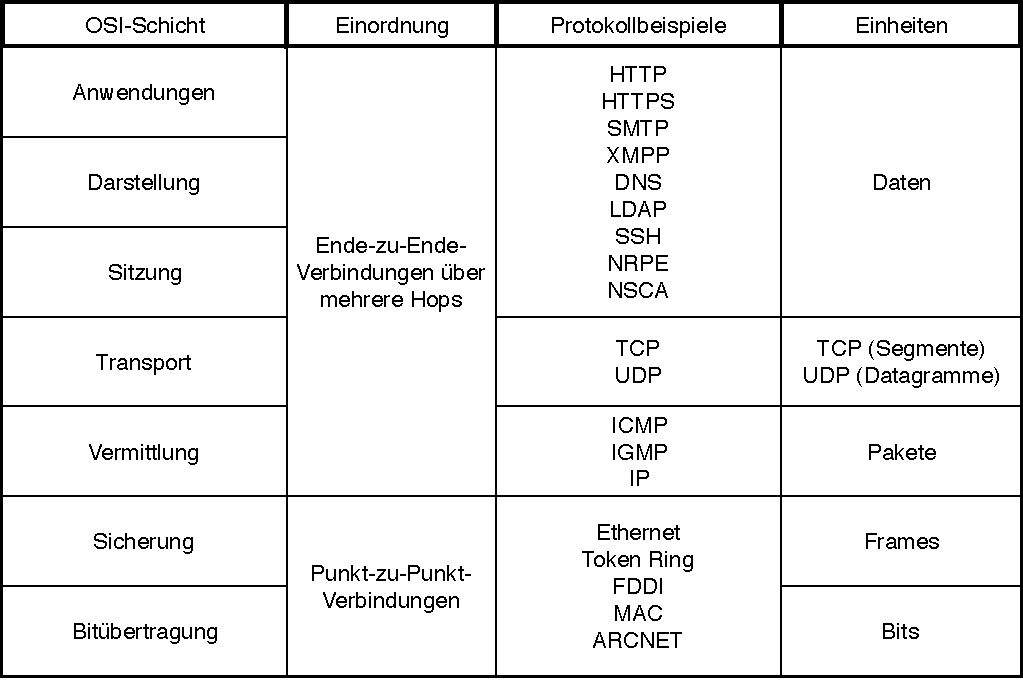
\includegraphics[width=0.8\textwidth]{figures/osi.pdf}
    \caption{Das OSI-Schichtenmodell mit Protokollbeispielen und
    verwendeten Einheiten}\label{fig:osi}
\end{figure}
\section*{\glsfirst{dns}}
\addcontentsline{toc}{section}{\glsfirst{dns}}
Aus Erfahrungen mit dem Internetvorgänger \gls{arpanet} wurde
abgeleitet, dass ein manuelles Eingeben von \gls{ip}\hyp{}adressen mit
steigender Anzahl von Knoten im Netzwerk immer unübersichtlicher wurde.
Hinzukommend sind \gls{ip}\hyp{}Adressen für den Menschen schwer zu
merken. Mit dieser Problemstellung als Grundlage arbeitete der Ingenieur
Peter Mockapetris an einem ersten Lösungsansatz: \glsfirst{dns}.
Bei \gls{dns} handelt es sich um einen mehr als 20 Jahre alten
Verzeichnisdienst, welcher über das gleichnamige Protokoll für Menschen
merkbare Internetadressen auf \gls{ip}\hyp{}Adressen abbildet.
\gls{dns} wurde erstmalig im Jahr 1983 in den beiden \glspl{rfc}
\gls{rfc} 882\cite{RFC0882} und \gls{rfc} 883\cite{RFC0883} beschrieben.
Damals befanden sich die \gls{dns}\hyp{}Einträge, die Abbildungen von
lesbarer Adresse auf \gls{ip}\hyp{}Adresse, noch verteilt auf
allen Servern des frühen Internets und wurden vom \gls{nic} verwaltet
und mit dem Dateiübertragungsprotokoll \gls{ftp}
synchronisiert\cite{RFC1034}. In der damaligen Zeit stellte sich dies
als ein Flaschenhals für das Internet heraus, da die Anzahl der Server
im Netzwerk exponentiell zunahm. Deshalb wurden nur vier Jahre später
Überarbeitungen von \gls{dns} veröffentlicht. Diese Überarbeitungen
wurden in den \glspl{rfc} 1034 und 1035 erläutert
und bilden die Grundlage für \gls{dns} wie es heute bekannt ist und auch
eingesetzt wird. Der heutige Ansatz verläuft dezentraler, als es damals
der Fall gewesen ist. Anstatt die \gls{dns}\hyp{}Einträge auf allen
Knoten des Internets zu verteilen und zentral vom \gls{nic} aus zu
steuern, existieren heute mehrere hierarchische Verwaltungsebenen. Dazu
wird der \gls{fqdn} hierarchisch gegliedert. Ein Beispiel für einen
\gls{fqdn} ist \emph{akira.rz.tu-clausthal.de}. Die
\autoref{fig:dnsname} veranschaulicht die Gliederung dieses \gls{fqdn} in die
einzelnen Bestandteile.
\begin{figure}[H]
    \centering
    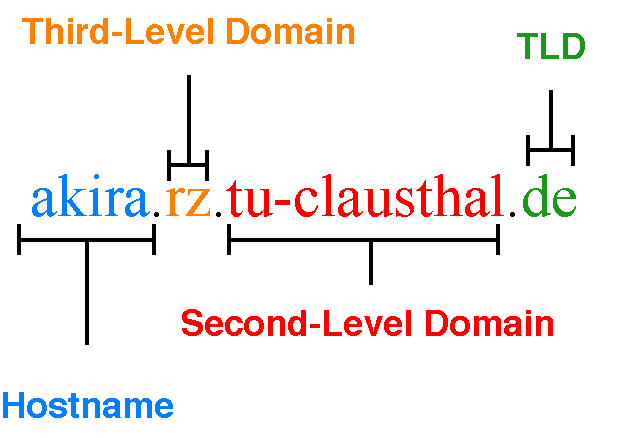
\includegraphics[width=0.5\textwidth]{figures/dnsname.pdf}
    \caption{Bestandteile eines \gls{fqdn} mit optionalem Hostname und Third-Level
    Domain}\label{fig:dnsname}
\end{figure}
Eine Angabe des Hostname oder einer Third-Level
Domain ist optional. Es können auch weitere Domains hinzugefügt werden.
So ist auch eine Sixth-Level Domain möglich. Die maximale Anzahl der
Subdomains ist in keinem der \gls{dns} \glspl{rfc} spezifiziert. Deshalb
ist die maximale Anzahl abhängig vom \gls{dns}\hyp{}Server, der die
Domains ausliefert. Nach \gls{rfc} 1035 ist die maximale Länge eines
\gls{fqdn} aber auf 255 Bytes begrenzt\cite[siehe Section
2.3.4]{RFC1035}, was die maximale Anzahl von Subdomains zumindest stark
einschränkt. Der Begriff Subdomain umfasst alle Domains unter der
\gls{tld}. \glspl{fqdn} sind nicht nur hierarchisch strukturiert, sondern
unterliegen zusätzlich einer Baumstruktur. Dessen Wurzel ist die
\emph{Root Domain}, meistens symbolisiert durch einen einfachen Punkt.
Eine Ebene direkt darunter sind die \glspl{tld}. Diese
werden in der Regel von den \glspl{nic} einzelner Länder verwaltet. Von
Ländern verwaltete \glspl{tld} haben meist Länderabkürzungen wie
\emph{de} (Deutschland), \emph{jp} (Japan) oder \emph{cn} (Volksrepublik
China). Es existieren aber auch militärische oder akademische
\glspl{tld} wie \emph{edu} und \emph{mil}. In Deutschland ist die DENIC eG
verantwortlich für Domains mit \emph{de}\hyp{}Endung.
In den letzten 5 Jahren kamen auch noch neue \glspl{tld} hinzu, welche
nicht an Länder geknüpft sind. Darunter fallen Markennamen wie
\emph{BMW}, \emph{Audi} oder \emph{Deutschepost} oder markenfreie Namen
wie \emph{academy}, \emph{fun} oder \emph{house}\cite{NEWTLDLIST}. Die
Vergabe der \glspl{tld} verlief direkt über die \gls{icann}. Der jeweilige
Käufer ist Eigentümer der jeweiligen \gls{tld}. Ein Eigentümer
einer \gls{tld} kann beliebig viele Subdomains erstellen für den
Eigenbedarf, diese weiterverkaufen oder gar verschenken. Weitere
wichtige Elemente des \gls{dns}\hyp{}Protokolls sind \emph{Name Server}
und \emph{Resolver}\cite[siehe Section 2.4]{RFC1034}.
\emph{Name Server} sind Server\hyp{}Programme, welche
Informationen zur Baumstruktur enthalten. Ergo halten \emph{Name
Server} Domain\hyp{}\gls{ip}\hyp{}Tabellen für ihre
hierarchische Ebene vor. Wenn kein Eintrag zu dem angefragten \gls{fqdn}
existiert, wird der nächsthöhere \gls{dns}\hyp{}Server gefragt. An
oberster Stelle stehen 13 \emph{Root Nameserver
Server}\cite{ROOTNAMESERVER}. Die \emph{Root
Name Server} umfassen die Namen und \gls{ip}\hyp{}Adressen aller
\emph{Name Server} die für die \gls{tld} verantwortlich sind.
\emph{Resolver} übernehmen die Rolle des Clients, sie senden
\gls{dns}\hyp{}Anfragen an \emph{Name Server}. Diese
Anfragen erfolgen in den meisten Fällen über das \gls{udp} an den Zielport
53\cite[Siehe Section 4.2.1]{RFC1035}. Es ist allerdings auch \gls{dns}
über \gls{tcp} spezifiziert\cite[Siehe Section 4.2.2]{RFC1035}.
Letzteres ist nötig für die \gls{dns}\hyp{}Erweiterungen
\gls{dns}\hyp{}over\hyp{}\gls{tls} (Port 853) und
\gls{dns}\hyp{}over\hyp{}\gls{https} (Port 443), welche das Protokoll \gls{dns} um
Verschlüsselung erweitern\cite{RFC7858}
(\gls{dns}\hyp{}over\hyp{}\gls{https} ist zum Zeitpunkt dieser Arbeit
noch nicht endgültig spezifiziert). Dieses Bestreben, \gls{dns} sicherer
zu machen, unterstreicht die Wichtigkeit des Protokolls. Das Protokoll
ist heute maßgeblich für das Funktionieren  des Internets. Ohne
\gls{dns} wären diverse vernetzte Anwendungen nicht möglich. Der
Webbrowser etwa löst permanent \gls{dns}\hyp{}Anfragen aus. Ist nur
eine dieser Anfragen fehlerhaft oder stark verzögert ist das für den
Nutzer augenblicklich zu merken. Im Fall von fehlerhaften Anfragen, wäre
eine Auflösung der Domain nicht möglich und eine Verbindung zu der
assoziierten \gls{ip}\hyp{}Adresse würde fehlschlagen. Der Webbrowser
würde in diesem Fall einen Fehlerbildschirm anzeigen.
Bei stark verzögerten
\gls{dns}\hyp{}Anfragen dauert der Aufbau einer neuen Seite 
länger als üblich. Wie wichtig schnelle Antwortzeiten eines Computers
sind, hat Walter Doherty bereits im Jahre 1982 mit seinem Paper \emph{The
Economic Value of Rapid Response Time} deutlich gemacht. Doherty
beobachtete einen signifikanten Anstieg an Benutzerinteraktionen, wenn
die Latenz der Anfrage (in diesem Fall bezogen auf normale
Computereingaben) unter einen bestimmten Wert fiel\cite{DOHERTY}.
Bezogen auf die Latenz von \gls{dns}\hyp{}Anfragen hieße das, dass der
Benutzer massiv bei seiner Arbeit ausgebremst wird. Dies führt nicht nur
zu Frustration beim Nutzer, sondern auch zu Verschwendung seiner
bezahlten Arbeitszeit und damit zu einer geringeren Produktivität.
\section*{\glsfirst{http}}
\addcontentsline{toc}{section}{\glsfirst{http}}
\glsfirst{http} ist ein auf \gls{tcp}/\gls{ip} aufbauendes
Datenübertragungsprotokoll, welcher auf der Andwendungsschicht des
\gls{osi} operiert. Der am meisten verbreiteste Anwendungszweck für das
Protokoll ist das Ausliefern von Webseiten über Port 80. \gls{http}
wurde erstmals im Jahre 1996 als \gls{rfc} 1945 spezifiziert, nachdem
es bereits fast sechs Jahre im Internet im Einsatz gewesen
war\cite{RFC1945}. Im Laufe der Jahre kamen weitere Versionen,
sowie diverse Erweiterungen für das Protokoll hinzu. Darunter
Erweiterungen für Kompression (um die Datenübertragungsrate zu erhöhen),
Verschlüsselung, Caching und Authentifikation. Seit 2015 ist die
aktuelle Version \gls{http}/2, welche in \gls{rfc} 7540 standardisiert
werden\cite{RFC7540}. \gls{http} ist ein zustandsloses Protokoll,
dementsprechend werden mehrere Anfragen getrennt voneinander und ohne
Kontext zu einander bearbeitet. Es wird keine Session aufgebaut und
keine Sitzungsinformationen verwaltet. Sitzungsinformationen können
zusätzlich durch \emph{Cookies} übertragen werden. \emph{Cookies}
ergänzen den \gls{http}\hyp{}Header um Sitzungsinformationen, dadurch
ist eine genaue Zuordnung möglich. Zur Interaktion mit dem Server
besitzt \gls{http} mehrere Methoden. Die häufigsten sind:
\begin{description}
    \item[GET] für einfache Anfragen
    \item[POST] um Informationen wie beispielsweise Logindaten an den
        Server zu senden.
    \item[HEAD] ähnlich wie \textbf{GET} mit dem Unterschied, dass
        der Server bei einer Antwort keinen Inhalt mitliefert.
\end{description}
Die Methoden \textbf{DELETE}, \textbf{PUT} sind nur für eine
\gls{restapi} relevant und umfassen das Löschen und hinzufügen. Um
herauszufinden, welche Methoden ein Server unterstützt, kann die Methode
\textbf{OPTIONS} verwendet werden.
Im \autoref{lst:httpanfrage} ist eine \gls{http}\hyp{}Anfrage mit Antwort und
Verbindungsaufbau an den Host \url{http://tu-clausthal.de}
visualisiert. Die eigentliche \gls{http}\hyp{}Anfrage beginnt ab Zeile 5
und endet in Zeile 9. Aus Zeile 5 wird ersichtlich, dass es sich um die
Version 1.1 von \gls{http} handelt und der Client via \emph{GET} den
Index der Seite \emph{tu-clausthal.de} (siehe Zeile 6) anfragt. Zeile 7
übermittelt den Namen und Version der Software mit, der diese
\gls{http}\hyp{}Anfrage gesendet worden ist und Zeile 8 definiert,
welche Mediatypen in einer Antwort erlaubt sind\cite{RFC2616}. Ab Zeile
10 beginnt die Antwort des Servers. Dort werden Protokoll und die
Version nochmal bestätigt und in diesem Beispiel ein Statuscode
hinzugefügt (301 weist daraufhin, dass der Inhalt der Seite verschoben
worden ist und an einem neuen Ort liegt (siehe Zeile 13)). Dazu wird auf
einen neuen \gls{url} verwiesen. Die \gls{url} dient als Pfadangabe zur
gewünschten Ressource oder Information. Bei \gls{http} haben diese
Pfadangaben den Präfix \emph{http://}. Zeile 11 gibt
das aktuelle Datum, die Uhrzeit und die Zeitzone an und Zeile 12 die
Software des Servers und deren Version. Die Zeilen 14 bis 16
enthalten die Information, dass der Server diverse Encodings unterstützt
(zum Beispiel Kompression mit dem Kompressionsalgorithmus \emph{gzip}),
die Länge des übermittelten Inhalts und der Typ des Inhalts sowie dessen
Zeichenkodierung. Die Zeilen 18 bis 21 enthalten den übermittelten
Inhalt, hier gekürzt dargestellt.
\begin{minipage}{\linewidth}
\begin{lstlisting}[caption={Eine HTTP-Anfrage an
http://tu-clausthal.de},label={lst:httpanfrage}]
* Rebuilt URL to: http://tu-clausthal.de/
*   Trying 2001:638:605:20:1::2...
* TCP_NODELAY set
* Connected to tu-clausthal.de (2001:638:605:20:1::2) port 80 (#0)
> GET / HTTP/1.1
> Host: tu-clausthal.de
> User-Agent: curl/7.59.0
> Accept: */*
>
< HTTP/1.1 301 Moved Permanently
< Date: Fri, 11 May 2018 23:48:50 GMT
< Server: Apache/2.2.22 (Ubuntu)
< Location: http://www.tu-clausthal.de/
< Vary: Accept-Encoding
< Content-Length: 235
< Content-Type: text/html; charset=iso-8859-1
<
<!DOCTYPE HTML PUBLIC "-//IETF//DTD HTML 2.0//EN">
<html><head>
[...]
</body></html>
* Connection #0 to host tu-clausthal.de left intact
\end{lstlisting}
\end{minipage}
Bei der Verwendung von \gls{http} können folgende Fehlerfälle auftreten:
\begin{itemize}
    \item Die Verbindung ist zu langsam und der Seitenaufbau erfolgt in
          einem für den Nutzer zu langsamen Tempo.
    \item Die Verbindung kommt nicht zu Stande, weil der Webserver nicht
          erreichbar ist.
\end{itemize}
\section*{\glsfirst{https}}
\addcontentsline{toc}{section}{\glsfirst{https}}
Bei \gls{https} handelt es sich um das Protokoll \gls{http} mit einer
zusätzlichen Schicht zur Verschlüsselung und Herstellung von
Datenintegrität. Dafür wird das Verschlüsselungsprotokoll \gls{tls}
benutzt, teilweise auch noch unter der Bezeichnung \gls{ssl} bekannt.
Dabei ist anzumerken, dass \gls{ssl} das Vorgängerprotokoll von
\gls{tls} ist.
Für den Verbindungsaufbau wird bei \gls{https} standardmäßig
Port 433 benutzt\cite[Siehe Section 2.3]{RFC2818}. Als
\gls{url}\hyp{}Präfix dient \emph{https://}. Bei der Verschlüsselung und
Herstellung der Datenintegrität bleibt die eigentliche
\gls{http}\hyp{}Syntax intakt, ergo handelt es sich um eine Verschlüsselung der
einzelnen \gls{http}\hyp{}Pakete. Dazu verschickt der Client beim
Verbindungsaufbau über Port 433 ein \emph{TLS ClientHello} an den
Server, woraufhin der \gls{tls}\hyp{}Handshake initiiert wird.
Dieser Handshake beinhaltet die Überprüfung der Integrität des Servers
unter Betrachtung des \gls{tls}\hyp{}Zertifikats. Das Zertifikat ist
ein öffentlicher Schlüssel, welcher mit einer
digitalen Signatur einer Zertifizierungsstelle beglaubigt worden ist.
Der Client besitzt eine Datenbank mit gültigen Zertifizierungsstellen
und vergleicht so das signierte Zertifikat des Servers mit dem
Zertifikat einer Zertifizierungsstelle. Wurden keine Mängel
festgestellt, beispielsweise ein abgelaufenes Zertifikat oder eine
fremde Zertifizierungsstelle, geht der Client davon aus, dass der Server
die Identität besitzt, die er vorgibt zu haben. Dies ist in so fern
problematisch, als in der Vergangenheit wiederholt bei
Zertifizierungsstellen eingebrochen worden ist und private Schlüssel zum
signieren von gültigen Zertifikaten gestohlen worden
sind\cite{PRIVATEKEYSSTOLEN}. Nach der Integritätsprüfung folgt der
eigentliche Aufbau einer verschlüsselten Verbindung. Für den Aufbau
existieren derzeit zwei mögliche Verfahren. Zum Einen der
\gls{rsa}\hyp{}Handshake und zum Anderen der
Diffie\hyp{}Hellman\hyp{}Handshake\cite{TLS}. Beim
\gls{rsa}\hyp{}Handshake wird vom Client ein symmetrischer Schlüssel
erzeugt, dieser wird mit dem öffentlichen Schlüssel des Servers
verschlüsselt und dem Server mitgeteilt. Der Server entschlüsselt den
symmetrischen Schlüssel unter Zuhilfenahme seines privaten Schlüssels.
Damit ist eine sichere Verbindung aufgebaut und der Client und der Server
sind in der Lage, sich mit dem symmetrischen Schlüssel
verschlüsselte Nachrichten zu senden. Beim
Diffie\hyp{}Hellman\hyp{}Handshake dagegen werden die öffentlichen
Schlüssel beider Gesprächspartner ausgetauscht und mit dem jeweiligen im
Besitz befindlichen privaten Schlüssel ein gemeinsamer symmetrischer
Schlüssel berechnet. Dieser symmetrische Schlüssel verlässt im Gegensatz
zum \gls{rsa}\hyp{}Handshake niemals den Server oder Client. Außerdem
ist es möglich, für jede Session einen neuen flüchtigen symmetrischen Key
zu erzeugen. Dies wird ermöglicht, in dem bei jeder neuen Session ein
neues Schlüsselpaar erzeugt wird. Ergo ist der
Diffie\hyp{}Hellman\hyp{}Handshake als sicherer anzusehen, da der
gemeinsame symmetrische Schlüssel niemals übertragen wird (auch nicht
verschlüsselt) und neue Sessions immer mit einem neuen Schlüssel
versehen werden. Letzteres ermöglicht \gls{pfs}. Durch \gls{pfs} ist es
einem Angreifer nicht möglich ältere aufgezeichnete Verbindungen zu
entschlüsseln, auch wenn er in den Besitz eines privaten Schlüssels
gelangt.
Die Fehlerfälle bei \gls{https} entsprechen denen von \gls{http}, 
erweitert um einige Fehler bezogen auf \gls{tls}:
\begin{itemize}
    \item Ein \gls{tls}\hyp{}Zertifikat ist ungültig
    \item Es kommt keine Verbindung auf Port 443 zustande, weil der
          Webserver kein \gls{https} unterstützt.
\end{itemize}
\section*{\glsfirst{cifs}}
\addcontentsline{toc}{section}{\glsfirst{cifs}}
\gls{cifs} ist ein von der Firma Microsoft 1996 eingeführtes
Datentransferprotokoll auf Basis von \gls{smb}\cite{SMBWIKI} und
\gls{netbios} über \gls{tcp}/\gls{ip}. Das Protokoll ist nicht nur auf
Dateitransfer beschränkt, sondern kann auch für Druckerfreigaben,
Windows-RPC (ein von Microsoft eingeführtes Protokoll, um Code aus der
Ferne auszuführen) und den NT-Domänendienst (ein von Microsoft
eingeführter Dienst zur Authentifizierung von Computern und Nutzern)
verwendet werden. Für die in dem vorherigen Kapitel genannte
Problemstellung ist allerdings nur der Dateitransfer via \gls{smb} von
Relevanz. Im Gegensatz zu \gls{http} ist \gls{cifs} ein
sessionbehaftetes Protokoll. Der \gls{cifs}\hyp{}Server ordnet also
jeder Verbindung eine Sitzung zu, die einem Client genau zugeordnet
werden kann. Darüber sind diverse Operationen möglich wie
Authentifizierung, Verschlüsselung oder \emph{Locking}\cite[S.
16]{MSSMB}. Beim \emph{Locking} wird der Zugriff auf eine Datei
beschränkt, um deren Korruption zu vermeiden, welche passieren kann, wenn
mehrere Nutzer auf die gleiche Datei schreiben. Um dies zu verhindern,
setzt der \gls{cifs}\hyp{}Server ein \emph{Lock} auf diese Datei und
lässt nur einen Client in diese Datei schreiben. Der eigentliche
Transfer der Dateien wird mit \gls{tcp} vor Korruption geschützt.
Die von der \gls{iana} für \gls{cifs} vergebene Portnummer ist:
445\cite[S. 19]{MSSMB}. Desweiteren hat \gls{tcp} den Vorteil, dass es
\emph{full-duplex} ist. \emph{Full-duplex} bedeutet, dass \gls{tcp} in
der Lage ist, gleichzeitig Daten zu empfangen und zu senden.
\autoref{fig:smbbytefield} zeigt den Aufbau eines solchen \gls{smb}\hyp{}Pakets mit
\gls{tcp}\hyp{}Header. Der Header beginnt mit einem Byte aus Nullen und
der anschließenden Länge des \gls{smb}\hyp{}Pakets. Danach folgt in
32\hyp{}Byte\hyp{}Blöcken die eigentliche Nachricht. Die Länge des Pakets wird als
drei Byte Integer in \emph{Network Byte Order} repräsentiert\cite[S.
21]{MSSMB}. \emph{Network Byte Order} entspricht dem \emph{Big Endian
Format}, bei dem das höchstwertige Byte zuerst gespeichert wird.
\begin{figure}[h]
    \centering
    \begin{bytefield}{32}
        \bitheader{0-31}\\
        \bitbox{8}{Null-Byte} & \bitbox{24}{Länge des SMB-Pakets}\\
        \bitbox{32}{SMB Nachricht}\\
        \bitbox{32}{\ldots}
    \end{bytefield}
    \caption{Aufbau eines \gls{smb}\hyp{}Pakets}\label{fig:smbbytefield}
\end{figure}
Bei der Verwendung von \gls{cifs} können folgende Fehlerfälle auftreten:
\begin{itemize}
    \item Die Verbindung zum Server, welcher den \gls{cifs}\hyp{}Share
          anbietet, weist eine hohe Latenz auf. Dies führt zu langsamen
          Schreib\hyp{} und Leseoperationen auf dem Share.
    \item Der \gls{cifs}\hyp{}Share ist nicht erreichbar.
\end{itemize}
\chapter*{Herleitung eines Lösungsansatzes}
\addcontentsline{toc}{chapter}{Herleitung eines Lösungsansatzes}
\section*{Anforderungsanalyse}
\addcontentsline{toc}{section}{Anforderungsanalyse}
Nachfolgend werden die ermittelten funktionalen und nichthyp{}funktionalen
Anforderungen erläutert. Funktionale Anforderungen stellen das
``eigentliche Systemverhalten und die jeweiligen Funktionen des zu
erstellenden Produkts''\cite[S. 20]{BPSE} dar, also die grundlegenden
Aufgaben der Software im Bezug auf die Problemstellung. Die
nichthyp{}funktionalen Anforderungen dagegen sind besonders. Sie umfassen
Anforderungen wie Sicherheit, nachträgliche Erweiterbarkeit,
Testbarkeit, also Anforderungen, welche erst nach der Entwicklung
mess\hyp{} oder testbar werden\cite[S. 292]{SNFA}. Um die funktionalen
und nichthyp{}funktionalen Anforderungen besser einordnen zu können, werden
folgende Schlüsselwörter zum Kennzeichnen für Anforderungen nach
\gls{rfc} 2119\cite{RFC2119} definiert:
\begin{description}
    \item[MUSS] ist eine absolute Anforderung an die Software. Alle
        Anforderungen, die mit \textbf{MUSS} markiert sind,
        \textbf{MÜSSEN} implementiert werden.
    \item[DARF NICHT] ist gleichbedeutend zu \textbf{VERBOTEN}.
    \item[SOLL] ist eine Anforderung, die implementiert werden
        \textbf{SOLLTE}, aber nicht \textbf{MUSS}. Dies ist der Fall bei
        Anforderungen, welche aus nachvollziehbaren Gründen nicht
        implementiert werden.
    \item[SOLL NICHT] ist gleichbedeutend zu \textbf{NICHT EMPFOHLEN}
        und beschreibt Anforderungen die nicht erfüllt werden sollten,
        wenn man sie vermeiden kann.
    \item[KANN] ist eine Anforderung die implementiert werden
        \textbf{KANN}. Diese Art von Anforderungen sind
        zusätzliches Extra und nicht nötig für die Grundfunktion der
        Software.
\end{description}
\textbf{Anmerkung}: Das \gls{rfc} 2119 ist im Original in Englisch. Ich
habe mich zur übersetzung der Schlüsselwörter auf die Übersetzung der
Schweizer Firma Adfinis SyGroup AG gestützt\cite{RFC2119DE}.
\subsection*{Funktionale Anforderungen}
\addcontentsline{toc}{subsection}{Funktionale Anforderungen}
\begin{center}
\begin{tabular}{p{0.7\textwidth-\tabcolsep}>{\raggedleft\arraybackslash}p{0.3\textwidth-\tabcolsep}}\toprule
    \textbf{FA1: Überwachung von \gls{dns} } & \textbf{Priorität: MUSS} \\\midrule
	\multicolumn{2}{p{\textwidth-\tabcolsep}}{%
        Die Software \textbf{muss} die Erreichbarkeit mehrerer
        \gls{dns}\hyp{}Server überprüfen können. Ebenfalls \textbf{muss} die
        Latenz einer \gls{dns}\hyp{}Anfrage gemessen werden können.}\\\bottomrule
\end{tabular}
    \captionof{table}{Funktionale Anforderung FA1}\label{table:FA1}
\end{center}
\begin{center}
\begin{tabular}{p{0.7\textwidth-\tabcolsep}>{\raggedleft\arraybackslash}p{0.3\textwidth-\tabcolsep}}\toprule
    \textbf{FA2: Überwachung von \gls{http} } & \textbf{Priorität: MUSS} \\\midrule
	\multicolumn{2}{p{\textwidth-\tabcolsep}}{%
        Die Software \textbf{MUSS} die Erreichbarkeit mehrerer
        \gls{http}\hyp{}Server überprüfen können. Ebenfalls
        \textbf{muss} die Latenz einer \gls{http}\hyp{}Anfrage gemessen werden können.}\\\bottomrule
\end{tabular}
    \captionof{table}{Funktionale Anforderung FA2}\label{table:FA2}
\end{center}
\begin{center}
\begin{tabular}{p{0.7\textwidth-\tabcolsep}>{\raggedleft\arraybackslash}p{0.3\textwidth-\tabcolsep}}\toprule
    \textbf{FA3: Überwachung von \gls{https} } & \textbf{Priorität: MUSS} \\\midrule
	\multicolumn{2}{p{\textwidth-\tabcolsep}}{%
        Die Software \textbf{MUSS} die Erreichbarkeit mehrerer
        \gls{https}\hyp{}Server überprüfen können. Ebenfalls \textbf{muss} die
        Latenz einer \gls{https}\hyp{}Anfrage gemessen werden können.}\\\bottomrule
\end{tabular}
    \captionof{table}{Funktionale Anforderung FA3}\label{table:FA3}
\end{center}
\begin{center}
\begin{tabular}{p{0.7\textwidth-\tabcolsep}>{\raggedleft\arraybackslash}p{0.3\textwidth-\tabcolsep}}\toprule
    \textbf{FA4: Überwachung von \gls{cifs} } & \textbf{Priorität: SOLL} \\\midrule
	\multicolumn{2}{p{\textwidth-\tabcolsep}}{%
    Die Software \textbf{MUSS} die Zeit messen können, die 
    zwischen einer \gls{cifs}-Abfrage und der Antwort von einem
    \gls{cifs}-Server} vergeht.\\\bottomrule
\end{tabular}
    \captionof{table}{Funktionale Anforderung FA4}\label{table:FA4}
\end{center}
\begin{center}
\begin{tabular}{p{0.7\textwidth-\tabcolsep}>{\raggedleft\arraybackslash}p{0.3\textwidth-\tabcolsep}}\toprule
    \textbf{FA5: Speicherung von Performance-Daten in einer Datenbank } & \textbf{Priorität: MUSS} \\\midrule
	\multicolumn{2}{p{\textwidth-\tabcolsep}}{%
        Das System \textbf{MUSS} die gesammelten Performance-Daten
        zur weiteren Auswertung an eine Datenbank übertragen.}\\\bottomrule
\end{tabular}
    \captionof{table}{Funktionale Anforderung FA5}\label{table:FA5}
\end{center}
\begin{center}
\begin{tabular}{p{0.7\textwidth-\tabcolsep}>{\raggedleft\arraybackslash}p{0.3\textwidth-\tabcolsep}}\toprule
    \textbf{FA6: Grafische Aufbereitung } & \textbf{Priorität: MUSS} \\\midrule
	\multicolumn{2}{p{\textwidth-\tabcolsep}}{%
        Die vom System zur Datenbank gesendeten Performance-Daten
        \textbf{MÜSSEN} für die Administratoren grafisch
        aufbereitet werden.
        Diese Graphen \textbf{MÜSSEN} via Port 80 (\gls{http})
        und Port 443 (\gls{https}) erreichbar sein.
        }\\\bottomrule
\end{tabular}
    \captionof{table}{Funktionale Anforderung FA6}\label{table:FA6}
\end{center}
\begin{center}
\begin{tabular}{p{0.7\textwidth-\tabcolsep}>{\raggedleft\arraybackslash}p{0.3\textwidth-\tabcolsep}}\toprule
    \textbf{FA7: Bandbreitenmessung } & \textbf{Priorität: MUSS} \\\midrule
	\multicolumn{2}{p{\textwidth-\tabcolsep}}{%
        Das System \textbf{MUSS} in der Lage sein Bandbreitenmessungen anhand des
        Durchsatzes vorzunehmen.
                }\\\bottomrule
\end{tabular}
    \captionof{table}{Funktionale Anforderung FA7}\label{table:FA7}
\end{center}
\begin{center}
\begin{tabular}{p{0.7\textwidth-\tabcolsep}>{\raggedleft\arraybackslash}p{0.3\textwidth-\tabcolsep}}\toprule
    \textbf{FA8: Native 1 Gigabit Ethernet Schnittstelle} & \textbf{Priorität: SOLL} \\\midrule
	\multicolumn{2}{p{\textwidth-\tabcolsep}}{%
    Die Hardware der Messpunkte \textbf{SOLL} über eine native 1 Gigabit
    Ethernet Schnittstelle verfügen.
    }\\\bottomrule
\end{tabular}
    \captionof{table}{Funktionale Anforderung FA8}\label{table:FA8}
\end{center}

\subsection*{Nicht-funktionale Anforderungen}
\addcontentsline{toc}{subsection}{Nicht-funktionale Anforderungen}
\begin{center}
\begin{tabular}{p{0.7\textwidth-\tabcolsep}>{\raggedleft\arraybackslash}p{0.3\textwidth-\tabcolsep}}\toprule
    \textbf{NFA1: Wahl der Programmiersprache} & \textbf{Priorität: SOLL} \\\midrule
	\multicolumn{2}{p{\textwidth-\tabcolsep}}{%
        Das System \textbf{SOLL} in einer dem Rechenzentrum der
        \gls{tuc} gängigen Programmiersprache entwickelt werden.
        Folgende Programmiersprachen werden im Rechenzentrum der
        \gls{tuc} täglich benutzt:
        \begin{itemize}
            \item Python
            \item Bash
            \item PHP
            \item Javascript
        \end{itemize}
    }\\\bottomrule
\end{tabular}
    \captionof{table}{Nicht-Funktionale Anforderung NFA1}\label{table:NFA1}
\end{center}
\begin{center}
\begin{tabular}{p{0.7\textwidth-\tabcolsep}>{\raggedleft\arraybackslash}p{0.3\textwidth-\tabcolsep}}\toprule
    \textbf{NFA2: Niedrige Beschaffungskosten} & \textbf{Priorität: SOLL} \\\midrule
	\multicolumn{2}{p{\textwidth-\tabcolsep}}{%
    Die Hardware der Messpunkte \textbf{SOLL} möglichst günstig in der Beschaffung
    sein.
    }\\\bottomrule
\end{tabular}
    \captionof{table}{Nicht-Funktionale Anforderung NFA2}\label{table:NFA2}
\end{center}
\begin{center}
\begin{tabular}{p{0.7\textwidth-\tabcolsep}>{\raggedleft\arraybackslash}p{0.3\textwidth-\tabcolsep}}\toprule
    \textbf{NFA3: Sicherheit} & \textbf{Priorität: SOLL} \\\midrule
	\multicolumn{2}{p{\textwidth-\tabcolsep}}{%
        Das System \textbf{SOLL} sicher konzipiert sein.
        Alle Übertragungen, welche sensible Daten übertragen,  \textbf{SOLLEN} mit gängigen
        als sicher eingestuften Algorithmen verschlüsselt sein.
        }\\\bottomrule
\end{tabular}
    \captionof{table}{Nicht-Funktionale Anforderung NFA3}\label{table:NFA3}
\end{center}
\begin{center}
\begin{tabular}{p{0.7\textwidth-\tabcolsep}>{\raggedleft\arraybackslash}p{0.3\textwidth-\tabcolsep}}\toprule
    \textbf{NFA4: Horizontale Skalierbarkeit} & \textbf{Priorität: MUSS} \\\midrule
	\multicolumn{2}{p{\textwidth-\tabcolsep}}{%
        Das zu entwickelnde System \textbf{MUSS} horizontal skalierbar
        sein.
        }\\\bottomrule
\end{tabular}
    \captionof{table}{Nicht-Funktionale Anforderung NFA4}\label{table:NFA4}
\end{center}
\begin{center}
\begin{tabular}{p{0.7\textwidth-\tabcolsep}>{\raggedleft\arraybackslash}p{0.3\textwidth-\tabcolsep}}\toprule
    \textbf{NFA5: Kontrollierbarkeit} & \textbf{Priorität: MUSS} \\\midrule
	\multicolumn{2}{p{\textwidth-\tabcolsep}}{%
        Das zu entwickelnde System \textbf{MUSS} bei wachsendem
        Komplexitätsgrad und Anzahl von Messpunkten steuerbar und
        kontrollierbar bleiben.
        }\\\bottomrule
\end{tabular}
    \captionof{table}{Nicht-Funktionale Anforderung NFA5}\label{table:NFA5}
\end{center}

\section*{Systemarchitektur}
\addcontentsline{toc}{section}{Systemarchitektur}
Auf Grundlage der Problemstellung und der Anforderungen ergibt sich die
folgende Aufstellung von Komponenten für die Systemarchitektur:
\begin{description}
    \item[Datenbank] Eine Datenbank zur Speicherung der
                     gewonnenen Messdaten.
    \item[Konfigurationsmanagement] Ein Subsystem zur Verwaltung, Kontrolle
        und Konfiguration der einzelnen Messsensoren, der Datenbank und
        der Visualisierungslösung.
    \item[Visualisierungslösung] Das Subsystem zur Visualisierung der, von
        den Messsensoren, gewonnenen Messdaten.
    \item[Messensor] Ein verteilter Messpunkt, um die in den
        Anforderungen spezifizierten Daten zu gewinnen.
\end{description}
Aus der Komponentenaufstellung ergeben sich die Assoziationen zwischen
den einzelnen Komponenten. Das Konfigurationsmanagement umspannt alle
Komponenten und sorgt für deren Konfiguration, Verwaltung und Kontrolle.
Die einzelnen Messensoren senden ihre Messdaten zur Datenbank. Der
Webserver mit der Visualisierungslösung stellt diese Daten für den Nutzer aufbereitet
 grafisch dar.
\begin{figure}[H]
    \centering
    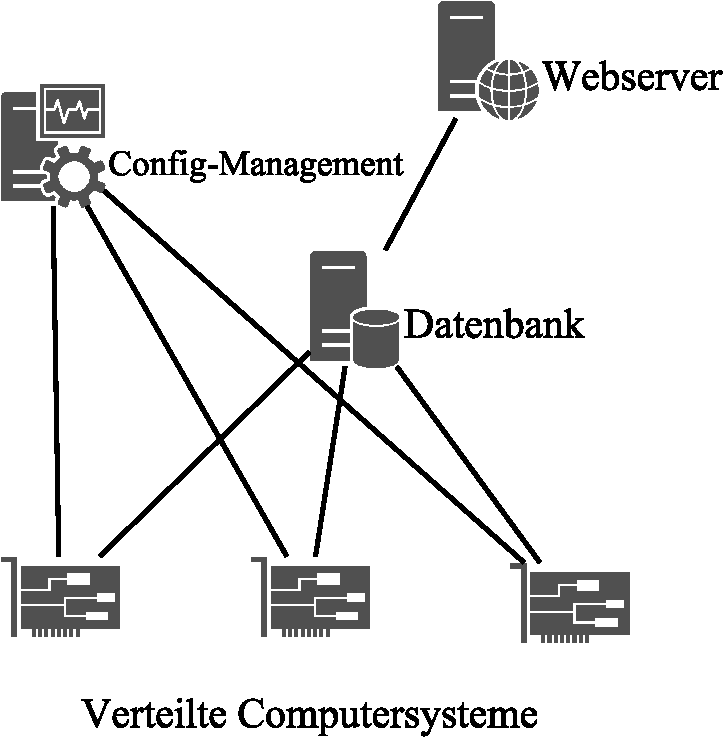
\includegraphics[width=0.8\textwidth]{figures/network.pdf}
    \caption{Zusammenspiel aller Systemkomponenten}\label{fig:network}
\end{figure}
\section*{Datenmodell}
\addcontentsline{toc}{section}{Datenmodell}
Zur Speicherung der Messdaten steht ein breites Spektrum von Datenbanken
zur Verfügung. Das Spektrum reicht von traditionellen, relationalen
Datenbanken, wie zum Beispiel MySQL, bis zu modernen
NoSQL\hyp{}Datenbanken, wie Key\hyp{}Value\hyp{}Stores und \glspl{tsdb}.
Dieses Kapitel versucht einen Überblick über alle Datenbanktypen zu
geben und den passenden Datenbanktyp für das Projekt festzulegen.
\subsection*{Relationale Datenbanken}
\addcontentsline{toc}{subsection}{Relationale Datenbanken}
Bei relationalen Datenbanken handelt es sich um tabellenbasierte Datensätze.
Als Grundlage dieser Datenbanken dienen Relationen.  Relationen sind
algrabische Strukturen und damit wohldefinierte Beschreibungen der
Tabellen. Also in sich selbst abgeschlossene Tautologien. Für Schreib\hyp{} und
Leseoperationen auf diesen durch Relationen beschrieben Tabellen wird eine
formale Sprache verwendet: die relationale Algebra. Jede Tabelle wird beim
Relationenmodell als eine Menge untergeordneter Tupel aufgefasst\cite[S.
4]{MEIER2013}. Ein weiteres Merkmal von relationalen Datenbanken ist die
Verwendung von Primärschlüsseln (Englisch: primary key). Durch Primärschlüsseln
ist jeder Eintrag in einer relationalen Datenbank eindeutig identifizierbar. Um
Datenbankeinträge abzufragen, zu manipulieren und in die Datenbank zu
transferieren, wird die international standardisierte
Datenbankbeschreibungssprache \gls{sql} eingesetzt. Die nachfolgende Tabelle
namens \emph{Studenten} beschreibt einen Datenbankeintrag in einer relationen
Datenbank:
\begin{center}
    \begin{tabular}{l c r}
        \toprule
        Matrikelnummer & Vorname & Nachname \\
        \midrule
        1              & Alice   & Alcatraz \\
        2              & Bob     & Bounty   \\
        3              & Charlie & Echo     \\
        \bottomrule
    \end{tabular}
\end{center}
In der oben abgebildeten Datenbank ist nur eine Tabelle namens
\emph{Studenten} vorhanden. Auf dieser Tabelle können mit \gls{sql} diverse
Operationen durchgeführt werden. \autoref{lst:sqlexample} zeigt das Hinzufügen neuer
Daten, das Abrufen von Daten, das Manipulieren von Daten und das
Erzeugen einer neuen Tabelle. Als Implementierung wurde \emph{sqlite}
verwendet. In der ersten Zeile wird durch das \emph{INSERT} Statement
ein neuer Student zur Tabelle \emph{Studenten} mit der Matrikelnummer 4,
dem Vornamen Dana und dem Nachnamen Foxtrott hinzugefügt. In der zweiten
Zeile werden alle Vornamen aus der Tabelle \emph{Studenten}
ausgegeben und in der siebten Zeile wird der Nachname vom Studenten
namens Charlie zu Alcatraz geändert. Zeile 8 zeigt das Erzeugen einer
neuen Tabelle \emph{Professoren} mit der MitarbeiterID als
aufsteigenden Primärschlüssel und den Einträgen zu Vorname und Nachname.

\begin{minipage}{\linewidth}
\begin{lstlisting}[caption={Verwendung von Structured Query Language},label={lst:sqlexample}]
sqlite> INSERT INTO Studenten VALUES (4,'Dana','Foxtrott');
sqlite> select Vorname from Studenten;
Alice
Bob
Charlie
Dana
sqlite> UPDATE Studenten SET Nachname = "Alcatraz" WHERE Matrikelnummer = 3;
sqlite> CREATE TABLE Professoren(MitarbeiterID INTEGER PRIMARY KEY ASC, Vorname, Nachname);
\end{lstlisting}
\end{minipage}
Bekannte Implementierungen für relationale Datenbanken sind:
\begin{itemize}
    \item MySQL
    \item MariaDB
    \item Sqlite
\end{itemize}
\subsection*{NoSQL\hyp{}Datenbanken}
\addcontentsline{toc}{subsection}{NoSQL\hyp{}Datenbanken}
NoSQL\hyp{}Datenbanken sind zunächst ein grober Sammelbegriff für alle
Datenbanken die kein relationales Konzept verfolgen und somit nicht
durch die Sprache \gls{sql} beschrieben werden können. In den meisten
Fällen handelt es sich bei NoSQL\hyp{}Datenbanken um einfache
Key\hyp{}Value\hyp{}Stores. Key\hyp{}Value\hyp{}Stores sind Ansammlungen
von Daten in Tupeln mit einem Schlüssel und einem Wert. Sie ähneln
demnach also einem Wörterbuch.  Meist sind diese Ansammlungen von Tupeln
in großen Binärdateien (\gls{blob}) oder sogar in einfachen Textdateien
gespeichert. Ein Beispiel für eine Key\hyp{}Value\hyp{}Datenbank ist
\emph{Dynamo} von der Firma \emph{Amazon}. Doch NoSQL\hyp{}Datenbanken
umfassen nicht nur Key\hyp{}Value\hyp{}Stores. Es existieren auch
NoSQL\hyp{}Datenbanken zum Speichern von Graphen, großen Mengen an
Dokumenten, wie \emph{IBM Notes}, Spaltenorientierten Datenbanken wie
\emph{Apache Cassandra} und der \glsfirst{tsdb}. \glspl{tsdb} kommen bei
jedem Gebiet zum Einsatz, wo große Mengen zeitlichabhängiger Daten
gespeichert werden müssen. \glspl{tsdb} sammeln große Datenmengen und
benutzen einen Zeitstempel als Index für diese Daten. Die gewonnenen
Daten werden demnach einem festen Zeitpunkt zugeordnet. Dies macht eine
\gls{tsdb} besonders beliebt als Datenbank für Wetterdaten,
Aktienhandelsdaten, Messdaten oder sonstige Daten die abhängig von der
Zeit und in besonders großen Mengen gespeichert werden sollen. Beispiele
für \glspl{tsdb} sind \emph{InfluxDB} und die \gls{tsdb} im
Monitoring-System \emph{Prometheus}. Trotz dieser Kategorisierungen
haben NoSQL\hyp{}Datenbanken mehrere gemeinsame Eigenschaften. So
verbindet sie der Verzicht von Eigenschaften relationaler Datenbanken
für höhere Skalierbarkeit\cite[S. 13]{TSDB}. Dadurch sind
NoSQL\hyp{}Datenbanken simpler aufgebaut und haben weniger Ansprüche an
die gespeicherten Daten. Es müssen keine Datentypen eingehalten oder
sonstige Relationen zwischen Daten gewährleistet werden. Alle Daten
werden in einer Tabelle gespeichert, welche sich beliebig horizontal
durch Verwendung von mehr Rechenzeit skalieren lässt. Dies äußert sich
in einer hohen Leistung, Skalierbarkeit und Flexibilität von
NoSQL\hyp{}Datenbanken\cite{NOSQL}.
\subsection*{Datenmodell}
Es werden folgende Informationen als Daten erwartet:
\begin{itemize}
    \item Ein sekundengenauer Zeitstempel.
    \item Der \gls{dns}\hyp{}Eintrag oder die
        \gls{ip}\hyp{}Adresse des Messknotens
    \item Die Messdaten
\end{itemize}
Da die Informationen nicht sonderlich komplex sind, bietet sich eine
NoSQL\hyp{}Datenbank für die Speicherung an. Eine NoSQL\hyp{}Datenbank
hat den Vorteil, dass sich die Datenbank einfacher skalieren lässt und
performanter ist. Durch die strikte Relation zwischen Messdaten und
ihrem sekundengenauen Zeitstempel fällt die Wahl auf eine \gls{tsdb}.
Folgende \gls{tsdb}\hyp{}Implementierungen stehen zur näheren Auswahl:
\begin{itemize}
    \item \emph{InfluxDB}\cite{INFLUXDB}
    \item \emph{OpenTSDB}\cite{OPENTSDB}
    \item \emph{Prometheus}\cite{PROMETHEUS}
\end{itemize}
\emph{InfluxDB} und \emph{OpenTSDB} sind beides generische Vertreter von
einer \gls{tsdb} und vielseitig einsetzbar. Interessant für dieses
Projekt ist jedoch \emph{Prometheus}. \emph{Prometheus} beschränkt sich
auf Monitoringdaten, bietet jedoch diverse Vorzüge gegenüber den anderen beiden
großen Vertretern von \glspl{tsdb} (Details zum internen Aufbau
und den Vorteilen von \emph{Prometheus} sind im Kapitel
\emph{Prometheus} zu finden). Daten werden in \emph{Prometheus} als
Tupel aus 64\hyp{}bit Fließkommazahlen und einem Millisekunden genauen
Zeitstempel gespeichert\cite{PROMETHEUS_DATA_MODEL}. Diese Tupel werden
mit einem Identifikator versehen. Dieser Identifikator besteht aus
einem eindeutigen Namen für die Metrik und einem
Key\hyp{}Value\hyp{}Store (siehe \autoref{lst:prometheusdataformat} Zeile 1; für ein
Beispiel siehe Zeile 2). Die Keys werden auch \emph{Labels} genannt.
Anhand dieser \emph{Labels} ist es möglich, Daten einer Metrik 
zu filtern. Zwei Stunden werden diese Metriken von \emph{Prometheus}
gesammelt bis sie, zusammen mit Metadaten und einer Indexdatei, in einem
Verzeichnis abgelegt werden. Metadaten sind Informationen über die
gesammelten Daten, darunter fallen \emph{Labels}. Die Indexdatei
speichert die Relation zwischen den Metriknamen und den Metriken, die
gestückelt abgelegt werden. Diese Stückelungen werden auch \emph{Chunks}
genannt\cite{PROMETHEUS_STORAGE}. Bevor diese Metriken gespeichert
werden, legt \emph{Prometheus} außerdem einen \gls{wal} an. Der \gls{wal}
dient zur Wiederherstellung von Daten nach einem Crash. Gelöschte Daten
werden nicht unwiderruflich gelöscht, sondern in
\emph{Tombstone}\hyp{}Dateien abgelegt. 
\autoref{lst:prometheusstorage} zeigt eine
solche Verzeichnisstruktur. Die \emph{Prometheus}\hyp{}Datenbank
arbeitet demnach dateibasiert im Gegensatz zu \glspl{blob} in
\gls{sql}\hyp{}basierten Datenbanken.
\emph{Prometheus}.
\begin{minipage}{\linewidth}
\begin{lstlisting}[caption={Prometheus Datenformat und
Beispiel},label={lst:prometheusdataformat}]
<metric name>{<label name>=<label value>, ...}
http_requests_total{service="service", server="www.tu-clausthal.de", env="production"}
\end{lstlisting}
\end{minipage}
\begin{minipage}{\linewidth}
\begin{lstlisting}[caption={Beispiel für das Prometheus Datenmodell},label={lst:prometheusstorage}]
./data/01BKGV7JBM69T2G1BGBGM6KB12
./data/01BKGV7JBM69T2G1BGBGM6KB12/meta.json
./data/01BKGV7JBM69T2G1BGBGM6KB12/wal
./data/01BKGV7JBM69T2G1BGBGM6KB12/wal/000002
./data/01BKGV7JBM69T2G1BGBGM6KB12/wal/000001
./data/01BKGTZQ1SYQJTR4PB43C8PD98
./data/01BKGTZQ1SYQJTR4PB43C8PD98/meta.json
./data/01BKGTZQ1SYQJTR4PB43C8PD98/index
./data/01BKGTZQ1SYQJTR4PB43C8PD98/chunks
./data/01BKGTZQ1SYQJTR4PB43C8PD98/chunks/000001
./data/01BKGTZQ1SYQJTR4PB43C8PD98/tombstones
./data/01BKGTZQ1HHWHV8FBJXW1Y3W0K
./data/01BKGTZQ1HHWHV8FBJXW1Y3W0K/meta.json
./data/01BKGTZQ1HHWHV8FBJXW1Y3W0K/wal
./data/01BKGTZQ1HHWHV8FBJXW1Y3W0K/wal/000001
./data/01BKGV7JC0RY8A6MACW02A2PJD
./data/01BKGV7JC0RY8A6MACW02A2PJD/meta.json
./data/01BKGV7JC0RY8A6MACW02A2PJD/index
./data/01BKGV7JC0RY8A6MACW02A2PJD/chunks
./data/01BKGV7JC0RY8A6MACW02A2PJD/chunks/000001
./data/01BKGV7JC0RY8A6MACW02A2PJD/tombstones
\end{lstlisting}
\end{minipage}
\section*{Prothemeus}
\addcontentsline{toc}{section}{Prometheus}
Bei \emph{Prometheus} handelt es sich um keine reine \gls{tsdb}.
\emph{Prometheus} ist vielmehr eine auf Monitoringdaten spezialisierte
und mit diversen Komponenten erweiterbare Monitoringanwendung. In diesem
Kapitel wird der interne Aufbau von \emph{Prometheus}, dessen
Komponenten und deren Zusammenspiel näher erläutert. \emph{Prometheus}
wurde ursprünglich im Jahr 2012 von Mitarbeitern des Online-Musikdiensts
\emph{Soundcloud} entwickelt\cite{PROMETHEUS_OVERVIEW} und im Jahr 2015
als Opensource Software freigegeben. \emph{Prometheus} entstand aus der
Not heraus, hunderte von Mikroservices und tausende von Service\hyp{}Instanzen
in einem firmeninternen Container\hyp{}Cluster zu
überwachen\cite{PROMETHEUS_YOUTUBE}. Seitdem setzt sich
\emph{Prometheus} besonders im Cloud\hyp{}Bereich durch und wurde 2016
sogar in die \emph{Cloud Native Computing Foundation}
aufgenommen\cite{CNCF}, einer Organisation zur Förderung von
Cloud\hyp{}Software im Opensource\hyp{}Bereich.
\subsection*{Komponenten}
\addcontentsline{toc}{subsection}{Komponenten}
Die meisten \emph{Prometheus}\hyp{}Komponenten sind in der Sprache
\emph{Go} (auch bekannt als \emph{Golang}) geschrieben. \emph{Go} ist
eine von der Firma \emph{Google} entwickelte, kompilierbare
Programmiersprache, welche sich vorallem dadurch auszeichnet, dass sie
sicherer als die Programmiersprache \emph{C} ist und eine gute
Portierbarkeit aufgrund von statischen Binärdateien besitzt. Durch diese
Eigenschaften setzt sich \emph{Go} immer stärker inbesondere im
Cloud\hyp{}Bereich durch\cite{INFOWORLD}. \emph{Prometheus}'
Kernkomponente ist der \emph{Prometheus Server}. Der \emph{Prometheus
Server} beinhaltet eine \gls{tsdb}, einen \gls{http}\hyp{}Server und ein
Modul zum Anfordern von Messdaten (im weiteren Verlauf
\emph{Retrieval} genannt). Die \gls{tsdb} wurde bereits im Kapitel
Datenmodell erläutert. Der \gls{http}\hyp{}Server bietet eine grafische
Oberfläche an, um Queries auf der \gls{tsdb} zu testen, inklusive
dem Anzeigen von Graphen. \autoref{fig:prometheuswebui} zeigt
die grafische Oberfläche mit einem Beispiel\hyp{}Query und Graphen.
Außerdem bietet der \gls{http}\hyp{}Server
eine \gls{restapi} an, an der die restlichen Komponenten andocken
können. Weitere Komponenten sind der \emph{Alertmanager}, das
\emph{Pushgateway}, die \emph{Exporter} und das bereits erläuterte und
im \emph{Prometheus Server} integrierte \emph{Prometheus Web UI}. Der
\emph{Alertmanager} ist verantwortlich für das Alarmieren der Benutzer,
wenn Messdaten, vom Benutzer bestimmte, Richtwerte überschreiten.
Unterstützt werden vom \emph{Alertmanager} direkt keine
Kommunikationswege. Viel mehr wird Fremdsoftware, beispielsweise für den
Mailtransfer, an den \emph{Alertmanger} angedockt. Das
\emph{Pushgateway} bietet einen statischen Bezugspunkt und Puffer, von dem der
\emph{Prometheus Server} mit dem \emph{Retrieval}\hyp{}Modul Messdaten
abholen kann. Dies ist nützlich, wenn der \emph{Prometheus Server}, statt
die Messdaten abzuholen, die Messdaten zugeschoben bekommen soll. Diese Messdaten
werden zum \emph{Pushgateway} geschoben und \emph{Prometheus
Server} holt die Messdaten dort ab. Weitere Komponenten sind die
\emph{Exporter}. \emph{Exporter} sind Applikationen, die die
Logik zum Sammeln von Messdaten besitzen und diese via einem
\gls{http}\hyp{}Server dem \emph{Prometheus Server} zur Verfügung
stellen. Es gibt eine Vielzahl von
\emph{Exportern} und die Zahl ist stetig steigend. Prominente Beispiele
für \emph{Exporter} sind:
\begin{itemize}
    \item \emph{Node Exporter}
    \item \emph{Blackbox Exporter}
\end{itemize}
\emph{Node Exporter} werden auf Hosts platziert und liefern allgemeine
Messdaten über diesen Host. Außerdem werden diverse Services, die auf dem
Host laufen, automatisch erkannt und Messdaten für diese Services zur
Verfügung gestellt. Wenn beispielsweise ein \gls{http}\hyp{}Server auf
Port 80 dieses Hosts läuft, sammelt der sich auf dem Host befindliche \emph{Node
Exporter} automatisch Messdaten über den Service und bietet diese dem
\emph{Prometheus Server} über einen eigenen \gls{http}\hyp{}Server an.
Der \emph{Blackbox Exporter} andererseits baut zwar ebenfalls einen
\gls{http}\hyp{}Server als Quelle für den \emph{Prometheus Server} auf,
aber Daten werden nicht über lokale Services gesammelt. Stattdessen
werden von dem \emph{Blackbox Exporter} aus diverse Tests durchgeführt,
wie beispielsweise die Erreichbarkeit von Kerndiensten wie \gls{dns}.
Die \autoref{fig:prometheus} zeigt den internen Aufbau des
\emph{Prometheus Servers} und dessen Zusammenspiel mit den einzelnen
Komponenten. Alle Verbindungen außerhalb des \emph{Prometheus Servers}
sind \gls{http}\hyp{}Anfragen einer \gls{restapi}. Alle Komponenten sind
statische Binärdateien und geschrieben in der Sprache \emph{Go}.
\begin{figure}[H]
    \centering
    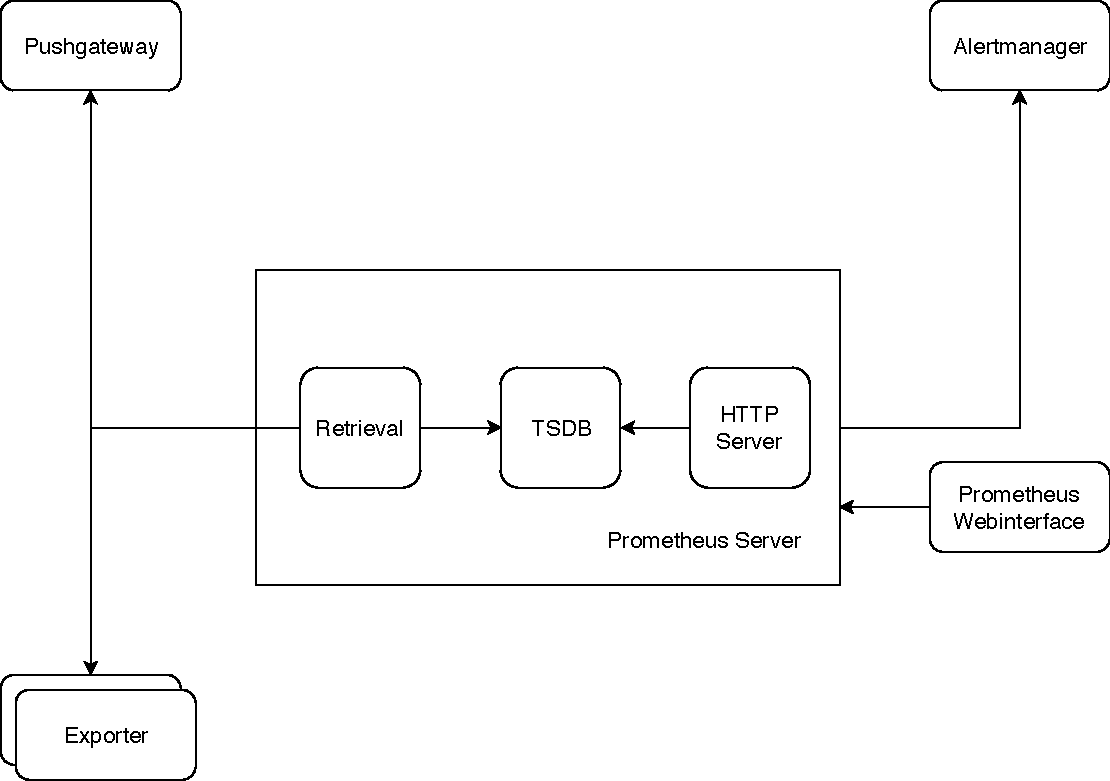
\includegraphics[width=1.0\textwidth]{figures/prometheus.pdf}
    \caption{Interner Aufbau des Prometheus Server und dessen
    Komponenten}\label{fig:prometheus}
\end{figure}
\begin{figure}[H]
    \centering
    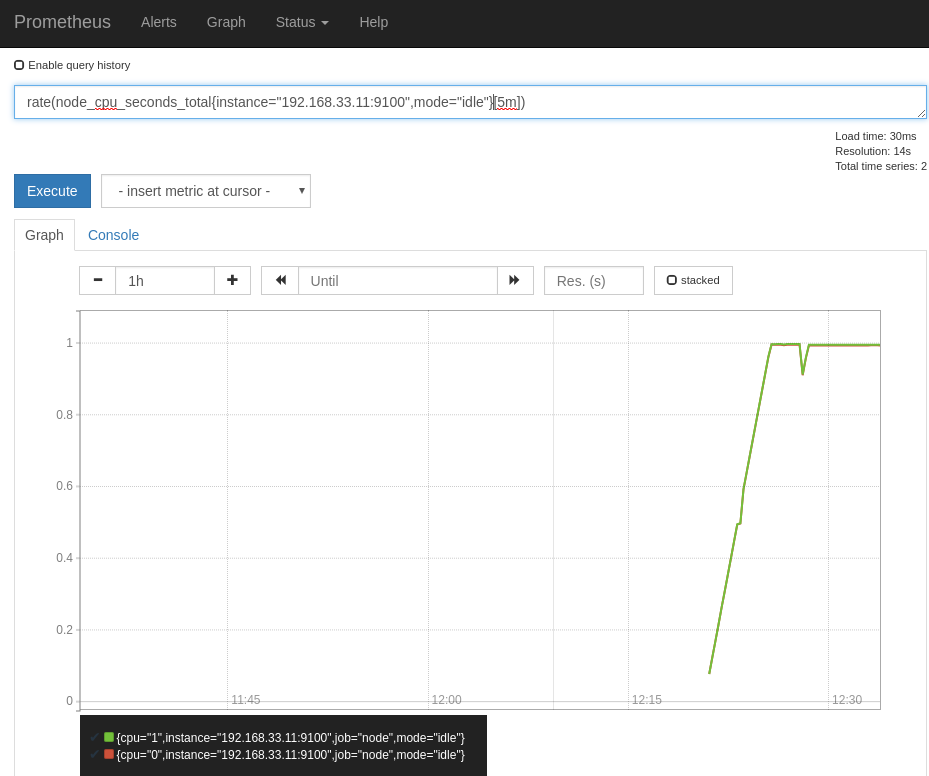
\includegraphics[width=1.0\textwidth]{figures/prometheus_web_ui.png}
    \caption{Prometheus Web UI Beispiel}\label{fig:prometheuswebui}
\end{figure}
\subsection*{PromQL}
\addcontentsline{toc}{subsection}{PromQL}
\emph{Prometheus} besitzt zum Abfragen der Messdaten eine eigene
Query\hyp{}Language names \emph{PromQL}. \emph{PromQL} ist nicht
vergleichbar mit \gls{sql} und besitzt keinen relationalen Ansatz.
Stattdessen handelt es sich um eine Art Filtersprache, welche mit
booleschen Operatoren und diversen Funktionen ergänzt worden ist.
Anhand von \emph{PromQL} lassen sich einzelne Messdatensätze auswählen
und weiter auswerten oder filtern\cite{PROMETHEUS_PROMQL}. Dies ist insbesondere für die
grafische Darstellung der Messdaten relevant. Dazu unterstützt die
\emph{PromQL} vier verschiedene Datentypen\cite{PROMETHEUS_PROMQL}:
\begin{description}
    \item[Instant Vector] ein Set von Messdaten mit demselben
        Zeitstempel.
    \item[Range Vector] eine Auswahl von Messdaten über einen größeren
        Zeitraum.
    \item[Scalar] ein Fließkommawert.
    \item[String] ein Array von Chars (zurzeit unbenutzt).
\end{description}
Der \emph{Instant Vector} besteht aus einem eindeutigen Namen, einer
Metrik und einem Key\hyp{}Value\hyp{}Store (siehe auch
\autoref{lst:prometheusdataformat}). Innerhalb eines \emph{Instant
Vectors} lassen sich reguläre Ausdrücke (Regex)
anwenden. Reguläre Ausdrücke beschreiben anhand von fest definierten
Zeichen und syntaktischer Regeln eine Menge von
Zeichenketten\cite{REGEXWIKI}. Für reguläre Ausdrücke verwendet
\emph{PromQL} die von der Firma \emph{Google} entwickelte Bibliothek
\emph{RE2}\cite{RE2}. Wird dieser \emph{Instant Vector} um einen
\emph{Range Selector} erweitert, handelt es sich um einen \emph{Range
Vector}. Ein \emph{Range Selector} ist eine in eckigen Klammern
geschriebene Zeitangabe für einen \emph{Instant Vector}. Der \emph{Range
Selector} wird dem \emph{Instant Vector} nachträglich angefügt.
Zusätzlich lassen sich diese Vektoren durch weitere Funktionen und
Operatoren beeinflussen. So bietet \emph{PromQL} eine Vielzahl von
weiteren Funktionen, um beispielsweise den Durchschnitt über einen
\emph{Range Vector} zu bilden\cite{PROMETHEUS_PROMQL_FUNCTIONS}.
\section*{Grafana}
\addcontentsline{toc}{section}{Grafana}
Da die \emph{Prometheus Web UI} eingeschränkt mit Graphen und
Visualisierung der Daten umgehen kann und eher eine Testplattform für
\emph{PromQL-Anfragen} darstellt, wird für den Zweck der
Visualisierung eine weitere Plattform verwendet:
\emph{Grafana}\cite{GRAFANA}. \emph{Grafana} zeichnet sich durch eine
hohe Erweiterbarkeit, vollen \emph{Prometheus}\hyp{}Support und einer
Vielzahl an Konfigurationsmöglichkeiten aus. Der Transport der Daten von
\emph{Prometheus} zu \emph{Grafana} findet via \gls{restapi} und der, von
\emph{Prometheus} unterstützten Query\hyp{}Language \emph{PromQL} statt
(\autoref{fig:prometheusgrafana} zeigt \emph{Grafanas} Platz in der
\emph{Prometheus}\hyp{}Landschaft).
\begin{figure}[H]
    \centering
    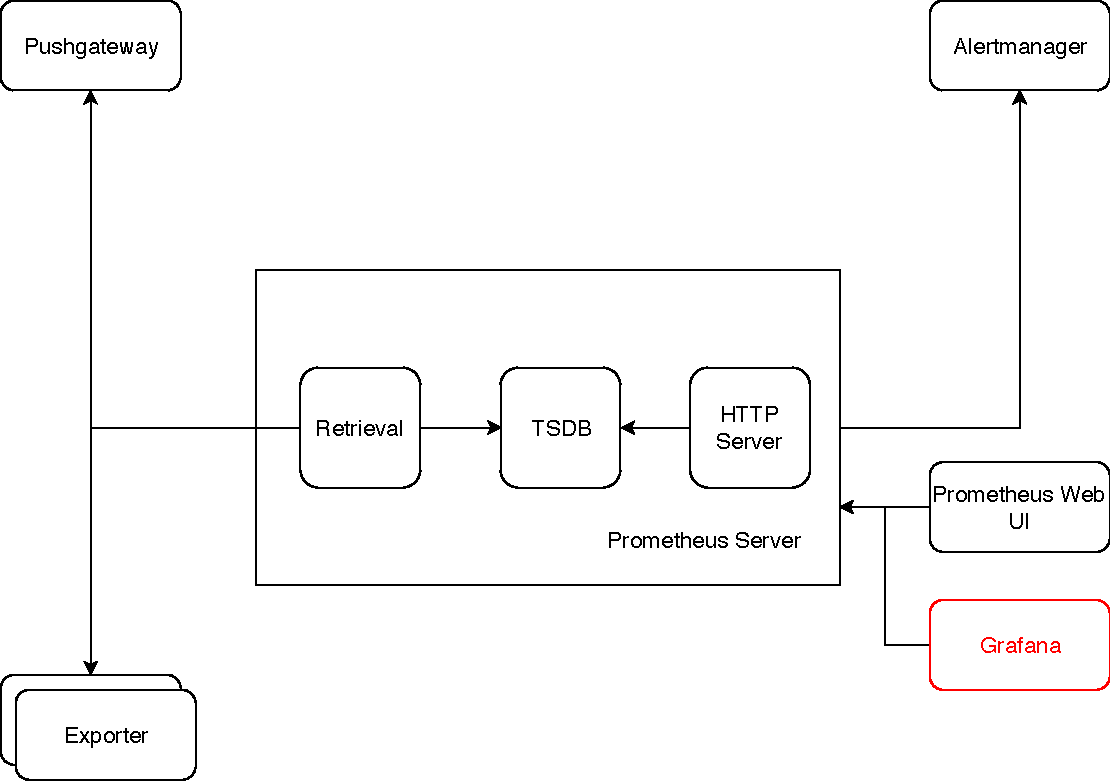
\includegraphics[width=1.0\textwidth]{figures/prometheus_grafana.pdf}
    \caption{Eingliederung von Grafana in Prometheus}\label{fig:prometheusgrafana}
\end{figure}
Ein weiteres Merkmal von \emph{Grafana} sind \emph{Grafanas}
Provisionierungseigenschaften. Durch diverse Einstellungen in
\emph{Grafanas} Konfigurationsdateien und Umgebungsvariablen lässt sich
Grafana gut in Cloud\hyp{}Umgebungen ausrollen (Umgebungsvariablen sind
temporäre oder permanente Variablen im Betriebssystem).
\section*{Konfigurationsmanagement}
\addcontentsline{toc}{section}{Konfigurationsmanagement}
In der Vergangenheit wurden Rechnersysteme zunehmend vertikal skaliert,
das heißt, die technischen Ressourcen des Rechnersystems wurden angehoben
(beispielsweise der \gls{ram}). In den letzten Jahren wurde zunehmends
festgestellt, dass diese Vorgehensweise nicht nur sehr kostenintensiv
ist, sondern auch nicht besonders zur Ausfallsicherheit beiträgt. Die
Antwort auf dieses Problem ist horizontale Skalierung. Bei horizontaler
Skalierung werden weitere Instanzen von Rechnersystemen der Anwendung
hinzugefügt. Dieser Ansatz ermöglicht ausfallsichere und äußerst
performante Infrastrukturen (zum Beispiel sind heutige Cloud\hyp{}Systeme
de facto alle horizontal skaliert). Diese horizontale Skalierung hat
allerdings auch andere Ansprüche. So wächst die Anzahl der zu
betreuenden Systemen rapide an.  Damals wurden solche Systeme noch von
Menschen gepflegt, konfiguriert und installiert. Durch die schiere Masse
der neuen Systeme ist das nun unmöglich und zu kostenintensiv geworden.
Daraufhin wurden Anwendungen ins Leben gerufen, welche die Arbeiten an
mehreren Systemen vereinfachen sollen. Die zwei Leitbegriffe für solche
Anwendungen sind \emph{Orchestrierung} und
\emph{Konfigurationsmanagement}. Bei der \emph{Orchestrierung} geht es
darum, eine hohe Anzahl von Systemen zu steuern, also gewisse Aufgaben
auf den jeweiligen Systemen anzustoßen.  \emph{Konfigurationsmanagement}
dagegen umfasst die Installation und Konfiguration der Systeme, im
englischsprachigen Raum zusammengefasst \emph{Deployment} genannt. Da im
Rechenzentrum der \gls{tuc} zur Zeit das auf der Programmiersprache
\emph{Python} basierende Orchestrierungs\hyp{} und
Konfigurationsmanagementwerkzeug \emph{Ansible} dominiert, beschränkt
sich diese Arbeit auf die Verwendung von \emph{Ansible}. Es gibt jedoch
andere populäre Werkzeuge. Darunter fallen beispielsweise
\emph{Puppet}, \emph{Saltstack} und \emph{Chef}.
\section*{Ansible}
\addcontentsline{toc}{section}{Ansible}
Die Entwicklung an \emph{Ansible} startete im Februar 2012 unter Michael
DeHaan als Opensource\hyp{}Anwendung\cite{ANSIBLE_ORIGINS}. Ein Jahr
später ging aus dem Projekt die Firma \emph{AnsibleWorks} hervor, welche
neben der Entwicklung von Ansible professionellen Support für die
Software anbietet und auch an einer webbasierten Benutzerschnittstelle
namens \emph{Tower} arbeitet\cite{ANSIBLEWORKS}. Im Jahr 2015 wurde die
Firma durch den großen Linux\hyp{}Dienstleister \emph{Red Hat}
übernommen\cite{ANSIBLEREDHAT}. Wenig später begann die
Opensource\hyp{}Gemeinschaft damit, \emph{Ansible} um unzählige Module zu
erweitern und so den Funktionsumfang zu vergrößern.
\subsection*{Funktionsweise}
\addcontentsline{toc}{subsection}{Funktionsweise}
\emph{Ansible} arbeitet mit Templates zur Orchestrierung und
Konfiguration von Systemen. Die Auszeichnungssprache für die
Datenstrukturen, welche die Templates befüllen, heißt \gls{yaml} (oft
auch nur mit YML abgekürzt). \gls{yaml} zeichnet sich durch für Menschen
einfache Lesbarkeit und die Möglichkeit, Kommentare einzufügen,
aus\cite{YAML_WIKI}. Außerdem besteht die Möglichkeit, in der
Programmiersprache \emph{Python} geschriebene Module mit in \gls{yaml}
aufgeschrieben Anweisungen zu nutzen. Diese Module sind quelloffen und
werden von einer Community um \emph{Ansible} und der Firma \emph{Red
Hat} gepflegt. Die zu pflegenden Systeme, nachfolgend nur noch als
Zielsysteme bezeichnet, sind in \emph{Ansible} in Gruppen zu
organisieren. Anhand vom Namen der Gruppe und des Zielsystems lassen
sich unterschiedliche vom Administrator definierte Daten laden. Diese
Daten werden in die mit \gls{yaml} verfassten Aufgaben eingefügt.
Auf diese Weise können komplexe Gebilde von Systemen abgebildet werden
und Gemeinsamkeiten in der Orchestrierung und Konfiguration effektiv ausgenutzt werden.
Bei einzelnen Konfigurationsdateien wird die auf \emph{Python} basierte Template\hyp{}Engine
\emph{Jinja2} benutzt\cite{JINJA2}. Durch \emph{Jinja2} lassen sich komplexe
Konfigurationsdateien auf den Zielsystemen in Form von Templates
ausdrücken. Das Ziel ist, ein Template für mehrere
Konfigurationsvarianten einer Konfigurationsdatei zu haben. Diese
Templates werden mit Datenstrukturen in \gls{yaml} gefüttert.
Um die Orchestrierung oder Konfiguration zu starten, reicht es, wenn sich
\emph{Ansible} auf dem System, welches zur Pflege eingesetzt werden
soll, befindet. Nachfolgend wird dieses System als Managementsystem
bezeichnet. Das Managementsystem verbindet sich zu den einzelnen
Zielsystemen via dem Protokoll \gls{ssh} und arbeitet die in
\gls{yaml}\hyp{}Dateien festgelegten Aufgaben ab. Dies geschieht durch
die Verwendung der Sprache \emph{Python} oder einfach durch Kommandos in
der entfernten Kommandozeile auf den Zielsystemen. Durch
diese Vorgehensweise arbeitet \emph{Ansible} \emph{agentless}, also ohne
einem Agenten auf dem Zielsystem. Dies
ermöglicht den Einsatz von \emph{Ansible} auch auf Systemen mit
eingeschränkter Erweiterbarkeit (beispielsweise Switches oder Router).
Außerdem arbeitet \emph{Ansible} idempotent, dadurch lassen sich
Aufgaben beliebig oft ausführen und führen immer zum gleichen Ergebnis.
\subsection*{Organisationsstruktur}
\addcontentsline{toc}{subsection}{Organisationsstruktur}
\emph{Ansible} hat eine definierte Struktur zur Speicherung der
Konfigurationsdateien, Aufgaben, Datenstrukturen für die Templates und
Templates. Dabei bedient sich \emph{Ansible} bei Wörtern aus der
Schauspielerei, um den Einstieg in die Software zu erleichtern.
\emph{Playbooks} (Deutsch: Drehbücher) werden verwendet, um einzelnen
Hosts \emph{Roles} (Deutsch: Rollen) zu zuweisen. Die nötigen Daten zum
Abspielen dieser Rollen befinden sich im \emph{Inventory} (Deutsch:
Inventar), zu dem die Hosts ebenfalls gehören. 
\autoref{lst:ansiblestructure} zeigt die Organisationsstruktur eines
solchen \emph{Ansible} Projekts. Die Datei \emph{ansible.cfg} ist die
Konfigurationsdatei für \emph{Ansible} und definiert den Pfad zum
Inventar, den Rollen und den \emph{Playbooks}. Die Datei \emph{hosts}
beinhaltet eine Auflistung aller Zielsysteme mit Eingliederung in
Gruppen und Subgruppen. Auf diese Weise lassen sich komplexe
Installationen aus Zielsystemen hierarchisch gliedern und
Gemeinsamkeiten fest machen. In den Dateien \emph{group\_vars} und
\emph{host\_vars} werden die eigentlichen Daten für die Gruppen und
einzelnen Hosts vermerkt. Der Ordner \emph{playbooks} umfasst alle
\emph{Playbooks}. Im Beispiel ist das \emph{Playbook}
\emph{configure\_hosts} abgebildet. Dies ist eine \gls{yaml}\hyp{}Datei.
\gls{yaml}\hyp{}Dateien werden häufig auch mit YML abgekürzt. Der
Ordner\emph{roles} beinhaltet die Rolle \emph{hello\_world} mit den
Unterordnern \emph{defaults}, \emph{files}, \emph{tasks} und
\emph{templates}. Im Ordner \emph{defaults} befinden sich
Standardbelegungen für Variablen zur Initialisierung. Der Ordner
\emph{files} umfasst statische Dateien, welche auf den Zielsystemen
installiert werden sollen. Die letzten beiden Ordner \emph{tasks} und
\emph{templates} umfassen die eigentliche Logik zur Konfiguration (die
abzuarbeitenden Aufgabenschritte) und \emph{Jinja2}\hyp{}Templates. Um
eine Konfiguration zu starten würde der Administrator das
\emph{Playbook} {configure\_hosts.yml} mit dem Kommando
\emph{ansible-playbook playbooks/configure\_hosts.yml} aufrufen.
\emph{Ansible} würde daraufhin das zu den Hosts gehörende Inventar
heraussuchen und die in den Rollen und Templates vorhandenen Variablen
durch Werte aus den \emph{host\_vars} oder \emph{group\_vars} ersetzen.
\begin{minipage}{\linewidth}
\begin{lstlisting}[caption={Organisationsstruktur eines Ansible
Projekts},label={lst:ansiblestructure}]
.
|-- ansible.cfg
|-- group_vars
|-- hosts
|-- host_vars
|-- playbooks
|   `-- configure_hosts.yml
`-- roles
    `-- hello_world
        |-- defaults
        |   `-- main.yml
        |-- files
        |   `-- static_file.txt
        |-- tasks
        |   `-- main.yml
        `-- templates
            `-- configuration.j2
\end{lstlisting}
\end{minipage}
\subsection*{Dateistruktur}
\addcontentsline{toc}{subsection}{Dateistruktur}
\emph{Ansible} nutzt als zentrale Dateistruktur die Auszeichnungssprache
\gls{yaml} und ergänzt diese durch Elemente der
Python\hyp{}Template\hyp{}Engine \emph{Jinja2}. \gls{yaml} unterstützt
gängige Datenstrukturen wie in etwa Listen und Wörterbücher
(Dictionaries) und Kombinationen davon sowie Kommentare. Höhere
Logikebenen werden durch \emph{Jinja2} erreicht (If/Else,
For\hyp{}Schleifen, While\hyp{}Schleifen etc). Dadurch ist \emph{Jinja2}
in der Theorie Turing-Vollständig. \autoref{lst:ansiblessh} ist ein
Beispiel für die Dateistruktur eines \emph{Ansible Tasks}. Der
\emph{Task} verteilt \gls{ssh}\hyp{}Schlüssel auf eine beliebige Anzahl
von Zielsystemen.  \gls{yaml}\hyp{}Dateien beginnen stets mit drei
Querstrichen und enden mit drei Punkten.  Mittlerweile ist dies jedoch
optional und \emph{Ansible} erkennt \gls{yaml}\hyp{}Dateien ohne diese
Markierungen (meistens an der Dateiendung \emph{.yml}). \emph{Ansible
Tasks} bestehen aus einer Liste von Dictionaries. Jeder Listeneintrag
stellt eine Aufgabe dar, welche \emph{Ansible} abzuarbeiten hat.
Initialisiert wird ein solcher Eintrag mit dem Namen der Aufgabe und
einer Abfolge von weiteren Schlüssel\hyp{}Wert\hyp{}Paaren. Bei den
Paaren handelt es sich um fest definierte und in Python verfasste
\emph{Ansible Module}. In dem Beispiel \autoref{lst:ansiblessh} sind
dies die Module \emph{file} und \emph{template}. Das
\emph{file}\hyp{}Modul dient zum Erstellen von Ordnern, platzieren von
statischen Dateien oder anlegen von Dateien mit statischen Inhalt.
Diesem Modul werden eine Anzahl von Parametern übergeben. In diesem Fall
ein Pfad auf einem Linux\hyp{}System, der gewollte Zustand
\emph{directory} sowie ein Besitzer, eine Gruppe und eine Konfiguration
der Dateiberechtigung. \emph{0700} bedeutet volle
Lese\hyp{},Schreib\hyp{} und Ausführrechte für den Besitzer der Datei
oder des Ordners. Dem zur Folge erstellt diese Zeile einen Ordner mit
den im vorherigen Satz erwähnten Dateirechten und dem Besitzer
\emph{root}. Das \emph{template}\hyp{}Modul hingegen liest ein lokales
\emph{Jinja2}\hyp{}Template ein, wertet dieses aus und hinterlegt es auf
dem Zielsystem mit den Dateirechten \emph{0600} (Schreib\hyp{} und
Leserechte) für den Benutzer \emph{root} in dem Pfad
\path{/root/.ssh/authorized\_keys}. \autoref{lst:ansiblejinja2}
zeigt das zum \emph{Task} gehörende \emph{Jinja2}\hyp{}Template. Die
erste Zeile im Template konfiguriert \emph{Jinja2} so, dass alle
Leerzeichen oder Tabs am Anfang einer Zeile gelöscht werden. In Zeile 2
ist der Anfang einer For\hyp{}Schleife in \emph{Jinja2}\hyp{}Syntax
abgebildet. In dieser For\hyp{}Schleife wird über die Liste
\emph{root\_ssh\_keys} iteriert und jede Iteration wird der Variable
\emph{user} als Wert zugewiesen. Der vertikale Strich startet einen
Filter. In diesem Fall der Filter \emph{sort}. Die Liste wird durch
diesen Filter vor dem Schleifendurchlauf sortiert. Der horizontale
Strich am Ende der Anweisung weist die Schleife an alle Leerzeichen oder
Tabs am Ende der generierten Zeile zu entfernen. Innerhalb der
For\hyp{}Schleife wird die Funktion \emph{lookup} aufgerufen, welche
eine Information auf dem lokalen Dateisystem einliest. Als Argument für
die Funktion wird angegeben, dass die Information aus einer Datei
bezogen werden soll und der Pfad zu dieser Datei wird aus der
\emph{user}\hyp{}Schleifenvariable und dem String \emph{../pubkeys/}
zusammengebaut. Die letzte Zeile beendet die Schleife. Gefüttert wird
dieses Template durch \autoref{lst:ansiblessh2}. 
\autoref{lst:ansiblessh2} wird dazu in den Ordnern \emph{group\_vars}
oder \emph{host\_vars} abgelegt und definiert die Liste
\emph{root\_ssh\_keys} mit den beiden Einträgen \emph{chris.pub} und
\emph{test.pub}
\begin{minipage}{\linewidth}
\begin{lstlisting}[caption={Beispiel eines Ansible Tasks},label={lst:ansiblessh}]
---

- name: ensure /root/.ssh exists
  file: path=/root/.ssh state=directory owner=root group=root mode=0700

- name: add authorized keys for root
  template: src=authorized_keys.j2 dest=/root/.ssh/authorized_keys owner=root group=root mode=0600

...
\end{lstlisting}
\end{minipage}
\begin{minipage}{\linewidth}
\begin{lstlisting}[caption={Beispiel eines Jinja2-Templates},label={lst:ansiblejinja2}]
#jinja2: lstrip_blocks: True

	{{ lookup('file', '../pubkeys/' + user) }}

\end{lstlisting}
\end{minipage}
\begin{minipage}{\linewidth}
\begin{lstlisting}[caption={Daten für das Jinja2-Template Beispiel},label={lst:ansiblessh2}]
---

root_ssh_keys:
  - chris.pub
  - test.pub

...
\end{lstlisting}
\end{minipage}
\subsection*{Sicherheit}
\addcontentsline{toc}{subsection}{Sicherheit}
\emph{Ansible} nutzt für alle Verbindungen das
Fernadministrationsprotokoll \glsfirst{ssh}. Dadurch ist die Integrität,
Sicherheit und Authentizität der übertragenen Daten sichergestellt.
\gls{ssh} verwendet dazu ein asynchrones Verschlüsselungsverfahren. Auf
dem Client wird ein Schlüsselpaar generiert. Üblicherweise durch moderne
kryptografisch sichere Verfahren wie \gls{rsa} oder Elliptischen Kurven.
Der öffentliche Schlüssel wird auf dem Zielsystem platziert, meistens
geschieht dies durch vorheriges Einloggen auf dem Zielsystem mit einem
Passwort. Bei der Verbindung vom Client zum Zielsystem wird durch das
asynchrone Verfahren die Authentizität des Servers und des Clients
bestätigt und der Zugriff gewährt. Um bestimmte Daten auch auf dem
lokalen Dateisystem des Managementsystems zu verschlüsseln wird
\emph{Ansible\hyp{}Vault} verwendet. \emph{Ansible\hyp{}Vault} ist ein
Mechanismus um Dateien mit einem symmetrischen Schlüssel zu
verschlüsseln. Als Algorithmus wird das Verschlüsselungsverfahren
\gls{aes} verwendet\cite{ANSIBLEVAULT}.
\section*{Wahl der Hardware}
\addcontentsline{toc}{section}{Wahl der Hardware}
Da das zu entwickelnde System horizontal skalierbar sein soll (siehe
Nicht-Funktionale Anforderung 4 (NFA4)) soll das System auch günstig in
der Anschaffung sein (NFA2). Dem kommt zu Gute, dass die Software auf den
Messpunkten nicht viele Hardware\hyp{}Ressourcen benötigt. Es wird
lediglich genug Speicher für ein kleines Linux mit einigen
Kernkomponenten wie \emph{openSSH} und der eigentlichen Software für die
Messpunkte benötigt. Durch die niedrigen Beschaffungskosten fallen somit
bereits größere Computersysteme in Form von Server\hyp{}Racks oder
Tower\hyp{}PC\hyp{}Einheiten weg. Übrig bleibt die Klasse der
Einplatinenrechner. Einplatinenrechner erfreuen sich in den letzten
Jahren immer größerer Beliebtheit und liegen in einem Budget\hyp{}Level
von \EUR{10} bis \EUR{100}. Nachfolgend werden die zwei Einplatinenrechner
\emph{Raspberry Pi 3B+} und \emph{Odroid XU4} verglichen.
Der \emph{Raspberry Pi 3B+} kommt mit folgenden Spezifikationen\cite{RASPI}:
\begin{itemize}
    \item SoC: Broadcom BCM2837B0 quad-core A53 (ARMv8) 64-bit @ 1.4GHz
    \item GPU: Broadcom Videocore-IV
    \item RAM: 1GB LPDDR2 SDRAM
    \item Netzwerk: Gigabit Ethernet (via USB channel), 2.4GHz and 5GHz 802.11b/g/n/ac Wi-Fi
    \item Bluetooth: Bluetooth 4.2, Bluetooth Low Energy (BLE)
    \item Speicher: Micro-SD
    \item GPIO: 40-pin GPIO header
    \item Anschlüsse: HDMI, 3.5mm analogue audio-video jack, 4x USB 2.0, Ethernet, Camera Serial Interface
        (CSI), Display Serial Interface (DSI)
    \item Dimensionen: 82mm x 56mm x 19.5mm, 50g Gewicht
    \item Preis: 32.88 Britische Pfund\cite{RASPI_PRICE} (\EUR{36.45} Stand: 2018-09-03)
\end{itemize}
Im Gegenzug dazu die \emph{Odroid XU4} Spezifikationen\cite{ODROID}:
\begin{itemize}
    \item SoC: Samsung Exynos5422 Cortex™-A15 2Ghz and Cortex™-A7 Octa core CPUs
    \item GPU: Mali-T628 MP6(OpenGL ES 3.1/2.0/1.1 and OpenCL 1.2 Full profile)
    \item RAM: 2Gbyte LPDDR3 RAM PoP stacked
    \item Netzwerk: Gigabit Ethernet, kein WLAN
    \item Bluetooth: nicht vorhanden
    \item Speicher: Micro-SD
    \item GPIO: 30-pin GPIO header\cite{ODROID_GPIO}
    \item Anschlüsse: 2x USB 3.0, 1x USB 2.0, HDMI 1.4a
    \item Dimensionen: 83mm x 58mm x 20 mm
    \item Preis: 59 US Dollar\cite{ODROID_PRICE} (\EUR{50,80} Stand: 2018-09-03)
\end{itemize}
\begin{figure}[H]
    \centering
    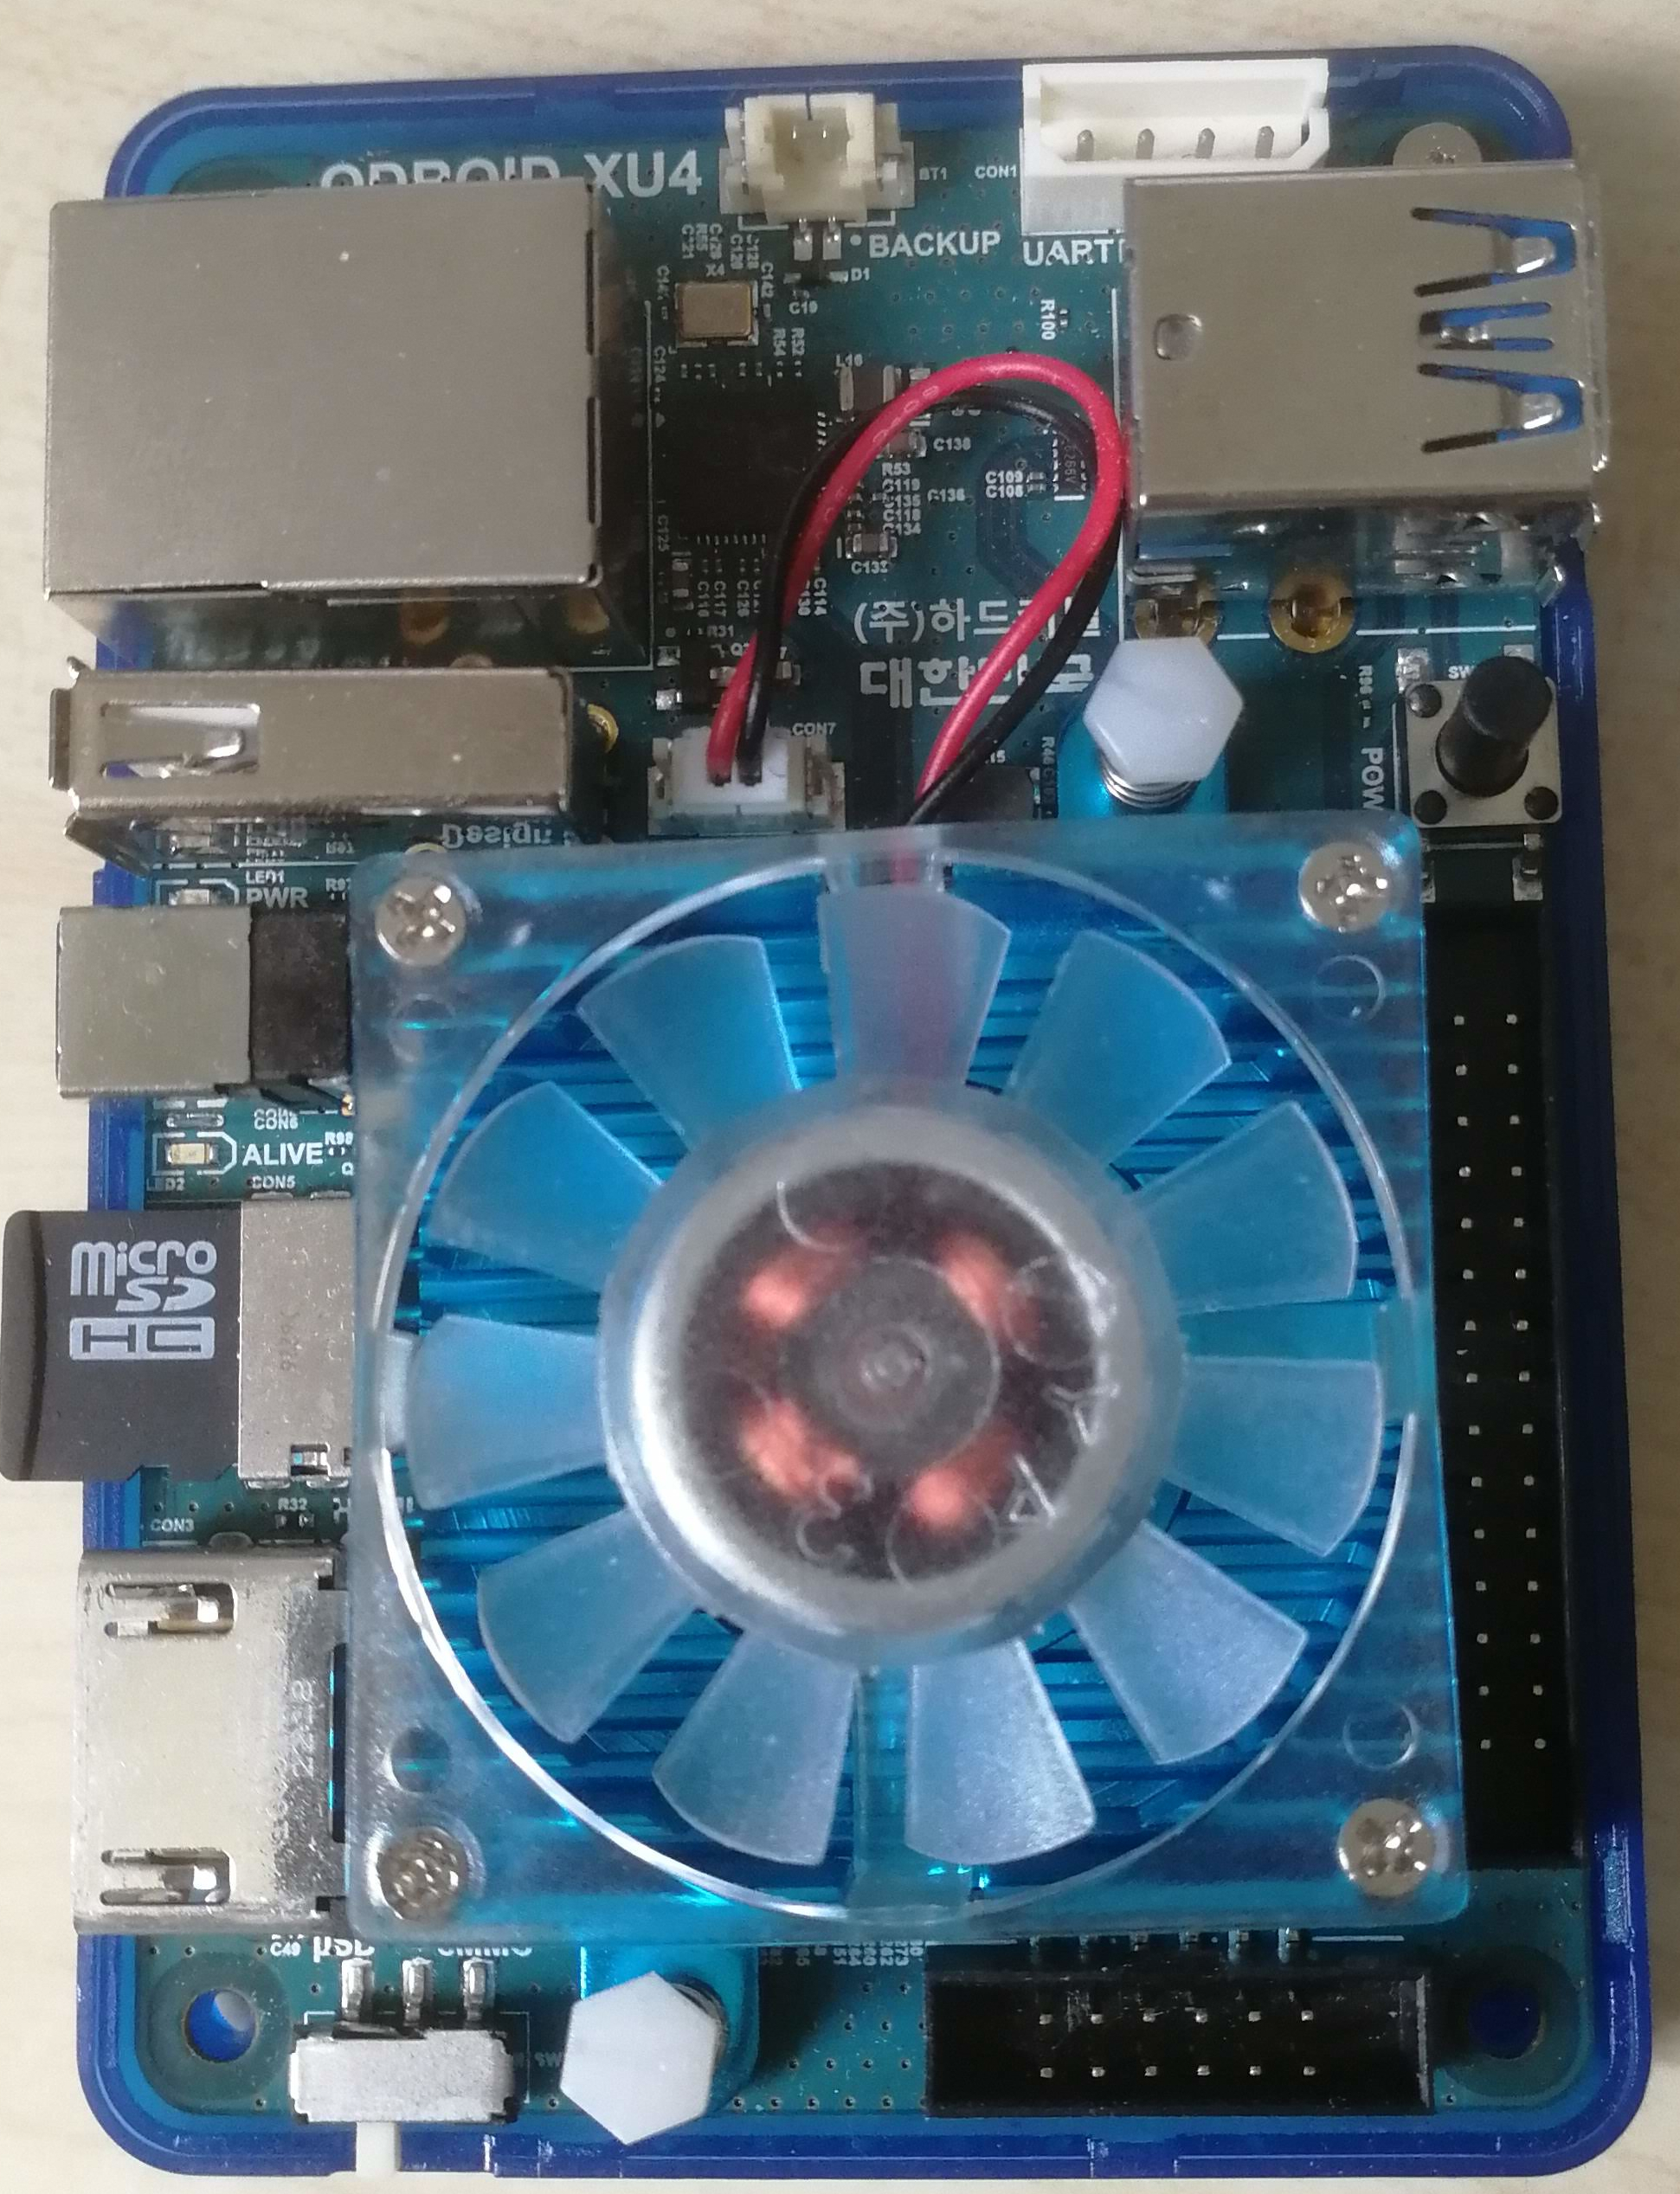
\includegraphics[width=0.5\textwidth]{figures/odroid.jpg}
    \caption{Darstellung eines Odroid XU4}\label{fig:odroid}
\end{figure}
\chapter*{Projektumsetzung}
\addcontentsline{toc}{chapter}{Projektumsetzung}
Die folgenden Unterkapitel umfassen die Umsetzung eines ersten
Prototyps. Dazu gehören das Erfüllen der Anforderungen, das Aufsetzen
eines ersten Test- und Entwicklungssystem, der Entwicklungsprozess
und der erste Prototype.
\section*{Erfüllung der Anforderungen}
\addcontentsline{toc}{section}{Erfüllung der Anforderungen}
Nachfolgend sind die evaluierten Anforderungen und deren Umsetzung
spezifiziert.
\tabulinesep=1.2mm
\begin{center}
    \begin{tabu}{X[-1] X}
\toprule
\textbf{Anforderung} & \textbf{Umsetzung}  \\
\midrule
        \hyperref[table:FA1]{\textbf{FA1}} & Die Überwachung von \emph{DNS} erfolgt durch den \emph{Prometheus} \emph{Blackbox-Exporter}. \\
        \hyperref[table:FA2]{\textbf{FA2}} & Die Überwachung von \emph{HTTP} erfolgt durch den \emph{Prometheus} \emph{Blackbox-Exporter}. \\
        \hyperref[table:FA3]{\textbf{FA3}} & Die Überwachung von \emph{HTTPS} erfolgt durch den \emph{Prometheus} \emph{Blackbox-Exporter}. \\
        \hyperref[table:FA4]{\textbf{FA4}} & \emph{Prometheus} ist zum Stand vom 01.09.2018 nicht in der Lage \emph{CIFS} zu überwachen. Um die Anforderung zu erfüllen wird der \emph{Prometheus} \emph{Node-Exporter} benutzt und die darunter liegende Bibliothek \emph{ProcFS} um Funktionalität erweitert. \\
        \hyperref[table:FA5]{\textbf{FA5}} & Die Performance-Daten werden in einer \emph{TSDB} in \emph{Prometheus} gespeichert. \\
        \hyperref[table:FA6]{\textbf{FA6}} & Die Grafische Aufbereitung erfolgt durch die Plattform \emph{Grafana}. \\
        \hyperref[table:FA7]{\textbf{FA7}} & Die Bandbreitenmessung erfolgt durch den \emph{Prometheus} \emph{Node-Exporter}. \\
        \hyperref[table:FA8]{\textbf{FA8}} & Wird erfüllt über die \emph{Odroid XU4} Plattform. \\
\bottomrule
    \end{tabu}
    \captionof{table}{Umsetzung der Funktionalen Anforderungen}
    \label{table:mapping1}
\end{center}
\tabulinesep=1.2mm
\begin{center}
    \begin{tabu}{X[-1] X}
\toprule
\textbf{Anforderung} & \textbf{Umsetzung}  \\
\midrule
        \hyperref[table:NFA1]{\textbf{NFA1}} & Das für das Deployment verwendete Projekt \emph{Ansible} benutzt \emph{Python}. Für die Erweiterung um \emph{CIFS}\hyp{}Support ist nur die Verwendung der Programmiersprache \emph{Golang} möglich. \\
        \hyperref[table:NFA2]{\textbf{NFA2}} & Die niedrigen Beschaffungskosten sind durch die Wahl der \emph{Odroid XU4} Plattform gegeben. \\
        \hyperref[table:NFA3]{\textbf{NFA3}} & Die für das Deployment benötigten Passwörter werden mit gängigen Verschlüsselungsverfahren in \emph{Ansible-Vault}  hinterlegt. Die Verbindungen zu den Zielsystemen finden verschlüsselt und mit einer Authentizitätsprüfung statt. \\
        \hyperref[table:NFA4]{\textbf{NFA4}} & Das System ist horizontal skalierbar durch den Einsatz von \emph{Prometheus} als Cluster einsetzbare Datenbank und \emph{Ansible} als Automatisierungswerkzeug zum Deployment. \\
        \hyperref[table:NFA5]{\textbf{NFA5}} & Das System bleibt kontrollierbar durch den Einsatz von \emph{Ansible}. \\
\bottomrule
    \end{tabu}
    \captionof{table}{Umsetzung der Nicht-Funktionalen Anforderungen}
    \label{table:mapping2}
\end{center}
\section*{Test- und Entwicklungssystem}
\addcontentsline{toc}{section}{Test- und Entwicklungssystem}
Da die benötigte Hardware zu Projektanfang noch nicht zur Verfügung
stand, galt es ein Test\hyp{} und Entwicklungssystem aufzubauen. Als
Grundlage für dieses Test\hyp{} und Entwicklungssystem dient die
Software \emph{Vagrant}\cite{VAGRANT} der Firma \emph{Hashicorp}. \emph{Hashicorp} ist
eine in San Fransisco im Jahr 2012 gegründete Firma, welche sich auf den
Einsatz und Entwicklung von Opensource Software
spezialisiert\cite{HASHICORP}. Der Fokus der Firma liegt auf
Automatisierung, Deployment und der Orchestrierung von
Softwaresystemen in der Cloud. Die Software ist auch ohne
eine Cloud\hyp{}Umgebung anwendbar. Für die Test\hyp{} und
Entwicklungsumgebung wird nur auf das Produkt \emph{Vagrant} der Produktpalette von
\emph{Hashicorp}, gemeinhin auch als \emph{Hashicorp-Toolchain} bekannt,
zurückgegriffen. Das Werkzeug \emph{Vagrant} bietet einen
Abstraktionsschicht über die gängigen Virtualisierungsplattformen wie in
etwa \emph{Virtualbox}, \emph{VMWare}, \emph{Qemu} aber auch über
Cloud\hyp{}Plattformen wie zum Beispiel \emph{Google Cloud},
\emph{Amazon AWS} und \emph{Openstack}. \emph{Vagrant} selbst ist eine
statisch gebaute aus \emph{Golang} kompilierte Binärdatei, dies
erleichtert das Deployment auf allen gängigen Systemen. Außerdem
zeichnet sich \emph{Vagrant} durch eine enge Verzahnung mit
Automatisierungswerkzeugen aus, darunter auch
\emph{Ansible}\cite{VAGRANT_DOCS}. \emph{Vagrant} abstrahiert die
Virtualisierungsplattform über einen \emph{Ruby}\hyp{}Interpreter. Es
wird eine Datei in der Programmiersprache \emph{ruby} angelegt, über
welche die Anzahl der virtuellen Maschinen und dessen Orchestrierung
organisiert wird. Diese \emph{Ruby} datei wird von \emph{Vagrant}
eingelesen und \emph{Vagrant} dockt über die APIs an den jeweiligen
\emph{Provider} an und spawned die virtuellen Maschinen. Der Dateiname
einer solchen Datei ist immer \emph{Vagrantfile}. \emph{Vagrantfiles}
sind austauschbar und ermöglichen so ein reproduzierbares und
automatisiertes Aufsetzen einer Testumgebung in wenigen Schritten. Ein
weiterer Grund für den Einsatz von \emph{Vagrant} ist die Vielzahl an
fertigen \emph{Images} (Speicherabbildern von Betriebssystemen). Anstatt
ein benötigtes Betriebssystem manuell in einer VM zu installieren ist es
möglich direkt über \emph{Vagrant} fertige \emph{Images} für gängige
Linux\hyp{}Distributionen zu ziehen. Dies beschleunigt den
Entwicklungsprozess ungemein, da der Entwickler sich voll auf die
Anwendung konzentrieren kann und seine Zeit nicht mit dem Installieren
von Betriebssystemen verschwendet. \autoref{lst:vagrantfile} zeigt
die \emph{Vagrantfile} zum erzeugen der Test\hyp{} und
Entwicklungsumgebung. In Zeile 1 wird eine For\hyp{}Schleife erzeugt,
welche 2 virtuelle Maschinen erzeugt. Die erste virtuelle Maschine trägt
den Namen \emph{puppetmaster} (Zeile 2) und wird mit einem \emph{Ubuntu
Bionic Beaver} (\emph{Ubuntu LTS 18.04}) konfiguriert (Zeile 3). \emph{Ubuntu} ist
ein Linux\hyp{}Derivat von der bekannteren Linux\hyp{}Distribution
\emph{Debian}. In Zeile 4 wird ein privates Netzwerk für die virtuelle
Maschine erzeugt. Die virtuelle Maschine bekommt demnach die
IP\hyp{}Adresse \textbf{192.168.33.10}. In den Zeilen 6 bis
einschließlich Zeile 8 wird eine zweite VM erzeugt und konfiguriert mit
dem Namen \emph{node1}, dem selben Betriebssystemabbild und der
IP\hyp{}Adresse \textbf{192.168.33.11}. Die virtuellen Maschinen liegen
beide im selben Netzwerk damit sie sich gegenseitig erreichen können.
Der Wirt\hyp{}Host auf dem die virtuellen Maschinen laufen ist ebenfalls
durch ein Interface zu den beiden Maschinen verbunden. Anhand dieser
\emph{Vagrantfile} ist es möglich die Testumgebung auf jedem System zu
starten auf dem \emph{Vagrant} installiert ist. Dazu muss lediglich die
\emph{Vagrantfile} in einen Ordner abgelegt werden und über die
Kommandozeile \emph{Vagrant} gestartet werden. Dies geschieht über das
Kommando: \emph{vagrant up}. \emph{Vagrant} lädt durch diesen Befehl das
benötigte Betriebssystemabbild herunter, konfiguriert die virtuellen
Maschinen mit dem Standard\hyp{}Provider \emph{Virtualbox} und
konfiguriert das Netzwerk für die Maschinen. Wenn die Maschinen
gestartet sind kann über den Befehl \emph{vagrant ssh <Name der vm>} auf
eine der virtuellen Maschinen über das Protokoll \gls{ssh} zugegriffen werden.
Durch diese Vorgehensweise lässt sich das Testsystem später auf jeden
anderen Hypervisor übertragen und die virtuellen Maschinen lassen sich
über den Befehl \emph{vagrant snapshot} leicht zu einem vorher
definierten Zustand zurücksetzen.
\begin{minipage}{\linewidth}
\begin{lstlisting}[caption={Vagrantfile der Test- und Entwicklungsumgebung},label={lst:vagrantfile}]
Vagrant.configure("2") do |config|
  config.vm.define "puppetmaster" do |puppetmaster|
    puppetmaster.vm.box = "ubuntu/bionic64"
    puppetmaster.vm.network "private_network", ip: "192.168.33.10"
  end
  config.vm.define "node1" do |node1|
    node1.vm.box = "ubuntu/bionic64"
    node1.vm.network "private_network", ip: "192.168.33.11"
  end
end
\end{lstlisting}
\end{minipage}
Bei der Anwendung des Befehls \emph{vagrant ssh} wird eine
Implementierung des \gls{ssh}\hyp{}Protokolls innerhalb \emph{Vagrants} benutzt. Um
die globale \gls{ssh}\hyp{}Implementierung zu verwenden ist es nötig den
von \emph{Vagrant} generierten privaten Schlüssel zu benutzen. Dieser
liegt im versteckten Verzeichnis: \path{.vagrant/machines/<VM
Name>/virtualbox/private\_key}. Dazu wird unter dem Betriebssystem
\emph{Linux} eine \gls{ssh}\hyp{}Konfigurationsdatei erstellt mit dem Pfad
\path{/home/<Benutzername>/.ssh/config}. \autoref{lst:sshconfig} zeigt
eine \gls{ssh}\hyp{}Konfigurationsdatei. Die erste Zeile vergibt einen
Alias für die gls{ip}\hyp{}Adresse. Auf diese Weise ist es nicht nötig
einen Eintrag im \gls{dns} vorzunehmen für ein Testsystem. Zeile 2
spezifiziert die Adresse nochmals. Zeile 3 definiert den Benutzer für
die \gls{ssh}\hyp{}Verbindung. Zeile 4 leitet die von \gls{ssh}
gespeicherten \emph{Fingerprints} für die \emph{Host-Zertifikate} nach
\path{/dev/null} um. \path{/dev/null} ist eie Gerätedatei innerhalb des
\emph{Linux}\hyp{}Betriebssystems zum Verwerfen von Daten\cite{DEVNULL}. Die
\emph{Fingerprints} der \emph{Host-Zertifikate} werden für die
Testsysteme verworfen, da bei jedem neu Erstellen die
Authentizitätsprüfung von \gls{ssh} sonst einen Fehler werfen würde.
Dies ist für Testzwecke unerwünscht. Zeile 5 schaltet die
Authentizitätsprüfung definitiv aus. Zeile 6 schaltet die
Passwort\hyp{}Authentifikation aus, da die Authentifikation nur über
private und öffentliche Schlüssel läuft. Zeile 7 gibt den
genauen Standort des privaten Schlüssels an. Zeile 8 konfiguriert
\gls{ssh} so, dass nur der angegebene private Schlüssel ausprobiert
wird und die letzte Zeile setzt das \emph{LogLevel} für Fehler auf eine
hohe Stufe. Dies erleichtert die Fehlersuche bei Problemen mit der
\gls{ssh}\hyp{}Verbindung.
\begin{minipage}{\linewidth}
\begin{lstlisting}[caption={Beispiel einer SSH Konfigurationsdatei},label={lst:sshconfig}]
Host puppetmaster 192.168.33.10
  HostName 192.168.33.10
  User vagrant
  UserKnownHostsFile /dev/null
  StrictHostKeyChecking no
  PasswordAuthentication no
  IdentityFile /home/chris/thesis/.vagrant/machines/puppetmaster/virtualbox/private_key
  IdentitiesOnly yes
  LogLevel FATAL

Host node1 192.168.33.11
  HostName 192.168.33.11
  User vagrant
  UserKnownHostsFile /dev/null
  StrictHostKeyChecking no
  PasswordAuthentication no
  IdentityFile /home/chris/thesis/.vagrant/machines/node1/virtualbox/private_key
  IdentitiesOnly yes
  LogLevel FATAL
\end{lstlisting}
\end{minipage}
\section*{Entwicklungsprozess}
\addcontentsline{toc}{section}{Entwicklungsprozess}
\subsection*{Versionsverwaltung}
\addcontentsline{toc}{subsection}{Versionsverwaltung}
Für den Entwicklungsprozess, des Konfigurationsmanagement und der
Erweiterung des Quellcodes von \emph{Prometheus} um \gls{cifs}, wird die
Versionsverwaltung \emph{Git} eingesetzt. \emph{Git} ist ein von Linus
Torvalds (dem Linux\hyp{}Chef\hyp{}Entwickler) entwickeltes dezentrales
Versionsverwaltungswerkzeug für Daten\cite{GITWIKI}. Eine
Versionsverwaltung hat den Vorteil, dass alle Entwicklungsschritte
chronologisch und inhaltlich nachvollziehbar sind und die Herkunft jedes
Entwicklungsschrittes klardokumentiert ist. Dazu werden die
Entwicklungsschritte möglichst atomar, also nicht weiter inhaltlich
zerlegbar, in das Versionsverwaltungswerkzeug zusammen mit Informationen
über den Entwickler und einer Beschreibung des \emph{Commits}, des
Entwicklungsschrittes, eingecheckt\cite{GITBOOK}. Die speziellen
Vorteile von \emph{Git} sind:
\begin{itemize}
    \item Ein Dezentraler Ansatz.
    \item Performance.
    \item Einfache Verwendung von \emph{Branches}, Entwicklungszweigen,
        um mehrere Entwicklungswege logisch zu trennen und später wieder
        zusammen zu führen.
    \item Opensource. Das Werkzeug \emph{Git} ist quelloffen und damit
        für jede Person einsehbar und erweiterbar.
\end{itemize}
Durch den dezentralen Ansatz muss der Entwickler nicht
\emph{online} sein um zu arbeiten. Auch ohne einen Internetzugang lässt
sich effektiv auf dem eigenen lokalen \emph{Repository}, den
Entwicklungsordner, arbeiten. Die Unterschiede zwischen den einzelnen
Revisionen oder \emph{Commits} werden, durch die lokale Speicherung als
\glspl{blob}, erfasst. Das gesamte \emph{Repository} kann auf einen oder
mehrere entfernte Server gesichert werden\cite{GITOTTO}. Außerdem kann
durch die Verwendung von \emph{Branches} (Deutsch: Zweige) die
Entwicklung von unterschiedlichen Funktionen zur selben Zeit erfolgen
ohne, dass die unterschiedlichen Entwicklungszweige (Englisch:
\emph{Feature Branch}) sich gegenseitig in
die Quere kommen. Ist die Entwicklung an der Funktion abgeschlossen wird
der Entwicklungszweig wieder mit dem ursprünglichen Hauptzweig (auch
\emph{Master} genannt) vereinigt. \autoref{lst:gitexample} zeigt einige
Beispiele für den \emph{Git Terminal Client}. In Zeile 1 wird das
\emph{Repository} von einem entfernten Server geklont und in Zeile 2
wird eine Datei des \emph{Repositories} verändert. Diese Veränderung
wird in Zeile 3 in die \emph{Staging}\hyp{}Ebene übernommen. Die
\emph{Staging}\hyp{}Ebene ist ein interner Bereich von \emph{Git} in dem
Änderungen am \emph{Repository} vorgemerkt werden\cite{PROGIT}. Mit dem
Kommando \emph{git commit} wird die Änderung in die Historie übernommen
und mit einem Kommentar des Autors versehen. \emph{git push} sendet die
Änderungen an einen oder mehrere entfernte Server. \emph{git log} zeigt
den Entwicklungsverlauf an. Es werden alle Änderungen erfasst mit
zusätzlichen Metadaten. Diese Metadaten beinhalten: die eindeutige
Nummer der Änderung, der Entwicklungszweig, der Name des Autors und
seine Email\hyp{}Adresse, ein Zeitstempel und ein Kommentar zu der
Änderung.
\begin{minipage}{\linewidth}
\begin{lstlisting}[caption={Beispiele für die Verwendung des
Git-Clients},label={lst:gitexample}]
$ git clone https://gitlab.rz.tu-clausthal.de/cre13/Ansible-Monitoring
$ vim ansible.cfg
$ git add ansible.cfg
$ git commit -m "ansible.cfg um weitere Optionen erweitert"
$ git push origin master
$ git log
commit 560920bb5f090aeb20a370b90472e45fba346417 (HEAD -> master)
Author: Christian Rebischke <christian.rebischke@tu-clausthal.de>
Date:   Tue Sep 25 17:07:50 2018 +0200

    ansible.cfg um weitere Optionen erweitert

[..]
\end{lstlisting}
\end{minipage}
\section*{Prototyp}
\addcontentsline{toc}{section}{Prototyp}
\section*{Betriebstests}
\addcontentsline{toc}{section}{Betriebstests}
\chapter*{Fazit}
\addcontentsline{toc}{chapter}{Fazit}
\nocite{*}
\printbibliography{}
\lstlistoflistings{}
\listoftables{}
\listoffigures
\printglossary{}
\end{document}
